\documentclass{article}
\usepackage[utf8]{inputenc}
\usepackage{amsthm}
\usepackage{amsmath}
\usepackage{amssymb}
\usepackage{graphicx}
\usepackage{float}
\graphicspath{ {./images/} }

\usepackage[noend]{algpseudocode}

\title{Algorithms and Data Structures Notes}
\author{William Guest}
\date{January 2023}

\theoremstyle{plain}
\theoremstyle{definition}
\newtheorem{thm}{Theorem}
\newtheorem{dummy}{Theorem}
\newtheorem{dummytwo}{Theorem}
\newtheorem{defn}[dummy]{Def}
\newtheorem{lemma}[dummytwo]{Lemma}

\renewcommand\algorithmicthen{}
\renewcommand\algorithmicdo{}

\begin{document}

\maketitle

\section{Amortized Analysis}
    Consider a sequence of operations in a data structure, with costs $c_1, \ldots, c_n, \ldots$. A worst case cost analysis would give an upper bound of
    \[ C = \max_{i=1,\ldots,n} c_1, \ldots, c_n \]
    Hence the total cost for the first $n$ operations is then $\leq Cn$. But some operations may be expensive and infrequent whilst others may be cheap and frequent. 
    \begin{defn}[Amortised Analysis]
        For a sequence of operations $c_1, \ldots, c_n$, we say that they have amortised cost $C$ if for every $i = 1, 2, \ldots, n$ we have that
        \[ c_1 + \ldots, + c_1 \leq Ci \]
    \end{defn}
    Another way to consider amortised analysis is
    \[ \max_i \frac{c_1 + \ldots + c_n}{i} \]
    We can think of the amortized cost as the average cost of each operation. 
    \subsection{Aggregate Method}
        In aggregate anaylsis, we determine an upper bound for the cost of $n$ operation, $T(n)$. The amortised cost is therefore $\frac{T(n)}{n}$, even when there are several types of operations in the sequence. 
    \subsection{Accounting Method}
        Also known as the "Banker's method", we assign "charges" to different operations, with some operations charged more or less than what they actually cost. We call the amount we charge an operation the \textbf{amortised cost}. When an operation's amortised cost exceeds the actual cost, this difference is known as the \textbf{credit}. This credit can help to pay for later operations. \\ \\
        In order to analyse the average cost per operation, we need to choose the amortised cost of each operation such that the total amortised cost is greater than or equal to the total actual cost, 
        (the amortized cost is an upper bound on the actual cost)
        i.e. for \textbf{all} sequences of n operations, 
        \[ \sum^n_{i=1} \hat{c_i} \geq \sum^n_{i=1} c_i \]
        where $\hat{c_i}$ is the amortised cost, and $c_i$ is the actual cost of the $i$th operation. This leads to the credit invariant
        \[ \sum^n_{i=1} \hat{c_i} - \sum^n_{i=1} c_i \geq 0 \]
        meaning that we must always have non-negative credit during the operation. 
    \subsection{Potential Method}
        Instead of representing prepaid work with "credit", which is stored with specific objects in the data structure, the potential method represents the prepaid work as "potential", which can also be released to pay for future operations. This potential is associated with the entire data structure, rather than specific objects within the data structure. \\ \\ 
        The potential is represented with a potential function, $\phi$ which maps a data structure to a real number. We start with the initial data structure $D_0$. For $i = 1, \ldots, n$, $c_i$ is the actual cost and $D_i$ is the data structure obtained from applying the $i$th operation to $D_{i-1}$. The amortised cost $\hat{c_i}$ is hence defined as 
        \[ \hat{c_i} = c_i + \phi(D_i) - \phi(D_{i-1})\]
        Hence the total amortized cost telescopes,
        \[ \sum^n_{i=1} \hat{c_i} = \sum^n_{i=1} c_i + \phi(D_0) - \phi(D_n) \]
        We then need to define $\phi$ such that $\phi(D_0) \geq \phi(D_n)$ so that the total amortised cost is an upper bound on the total actual cost. We usually define $\phi(D_0) = 0$, so we just need to show that for all n
        \[ \phi(D_n) \geq 0 \]
        A general rule of thumb is that more costly data structures should have a higher potential function. 
    
\section{Union Find}
    A disjoint-set data structure maintains a collection $F = \{ S_1, \ldots S_k \}$ of \textbf{disjoint} dynamic sets. We identify each set by a representative $rep(S)$, which is some member in the set. We want to define the following operations:
    \begin{itemize}
        \item MAKE-SET$(x)$ creates a new set whose only member and representative is $x$. (Note that as sets are disjoint, they can't be in any other set). 
        \item UNION$(x, y)$ unites the disjoint sets that contain $x$ and $y$. The representative of this new set is any member of $S_x \cup S_y$, typically $rep(S_x)$ or $rep(S_y)$. Sets $S_x$ and $S_y$ are removed from $F$ and $S_x \cup S_y$ is added to $F$. 
        \item FIND-SET$(x)$ returns a pointer to the representative of the set containing $x$
    \end{itemize}

    This algorithm is used in Kruskal's Algorithm for Minimum Spanning Trees
    \begin{algorithmic}[1]
            \State{$A = \emptyset$}
            \For{$v \in V$}
                \State{MAKE-SET(v)}
            \EndFor
            \State{Sort E into increasing order by weight w}
            \For{$(u, v) \in E$}
                \If{FIND-SET(u) $\neq$ FIND-SET(v)}
                    \State{$A = A \cup \{ (u, v) \}$}
                    \State{UNION($u,v$)}
                \EndIf
            \EndFor
        \end{algorithmic}

    There are three ways of implementing union find. 
    \subsection{Array Implementation}
        Suppose the elements are $1,\ldots, n$
        We maintain the representatives of each set in an array $R$.
        \begin{itemize}
        \item MAKE-SET$(x)$ - $R[x] = x$, time = $O(1)$
        \item UNION$(x, y)$ - scan R; if $R[i] = R[x], set R[i] := R[y]$, time = $O(n)$
        \item FIND-SET$(x)$ - return R[x], time = $O(1)$
        \end{itemize}
    \subsection{Linked List Implementation}
        In the linked list implementation, each set is represented by its own linked list. The object for each set has a \textit{head}, pointing to the first element in the list and a \textit{tail}, pointing to the last object. Each object in the list contains a member of a set, a pointer to the next item in the list and a pointer to the set object. The representative of the set is the first object in the list. 

        \begin{figure}
            \centering
            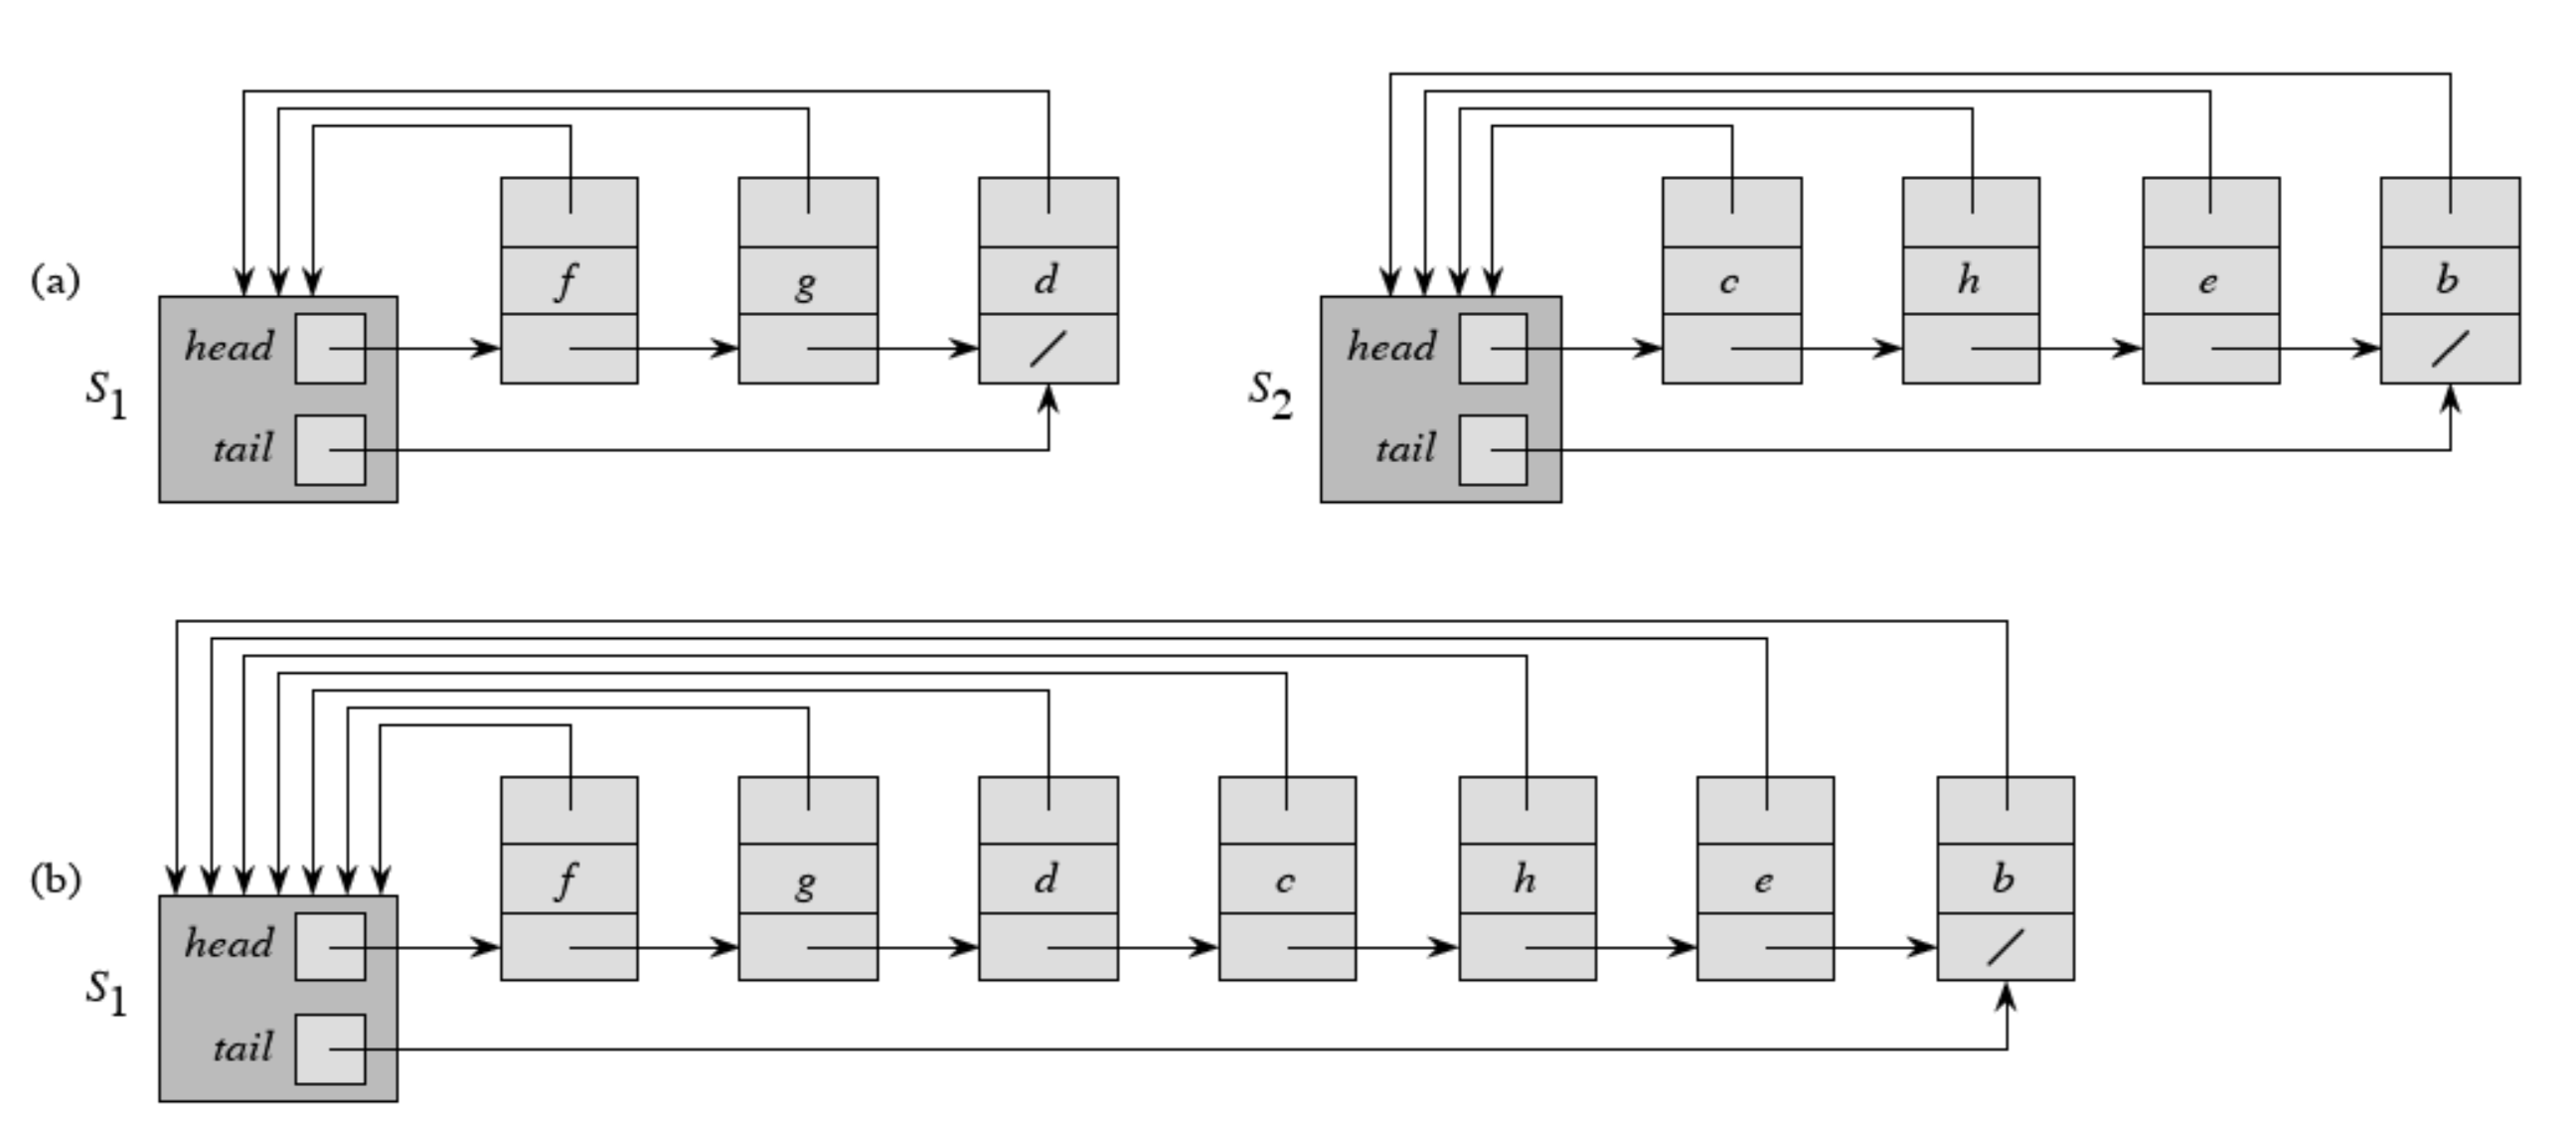
\includegraphics[width=\linewidth]{images/linkedlist.png}
            \caption{Before: $S_1$ and $S_2$; After $S_1 := S_1 \cup S_2$}
            \label{fig:linkedlist}
        \end{figure}

        \begin{itemize}
        \item MAKE-SET$(x)$ - Just create the set objects etc, time = $O(1)$
        \item UNION$(x, y)$ - We append the tail pointer for $x$'s list to the head of $y$'s list. We also need to change the set object pointer for each of the elements in $y$, time = $O(|S_y|)$
        \item FIND-SET$(x)$ - return the follow the pointer to the set object, which points to the representative of the list, time = $O(1)$
        \end{itemize}

        We can find a heuristic for UNION, we should always append the smaller tree to the longer tree. We do this by keeping track of the height of each tree in the root. Since each head is updated at most $log(n)$ times, the time taken is $O(m + n log n)$ for a sequence of $m$ operations on $n$ elements. 
        
    \subsection{Disjoint Set Forest}
        In the disjoint set forest implementation, we represent sets by rooted trees, with each node containing one element and each tree representing one set. The root of each tree is the representative of each set (and is hence its own parent).  

        \begin{itemize}
        \item MAKE-SET$(x)$ - Create a tree with one node, time = $O(1)$
        \item UNION$(x, y)$ - The root of $x$'s tree points to the root of $y$'s (or vice versa), time = $O(tree height)$
        \item FIND-SET$(x)$ - Follow parent pointers until we reach the root, time = $O(tree height)$
        \end{itemize}

        \begin{figure}
            \centering
            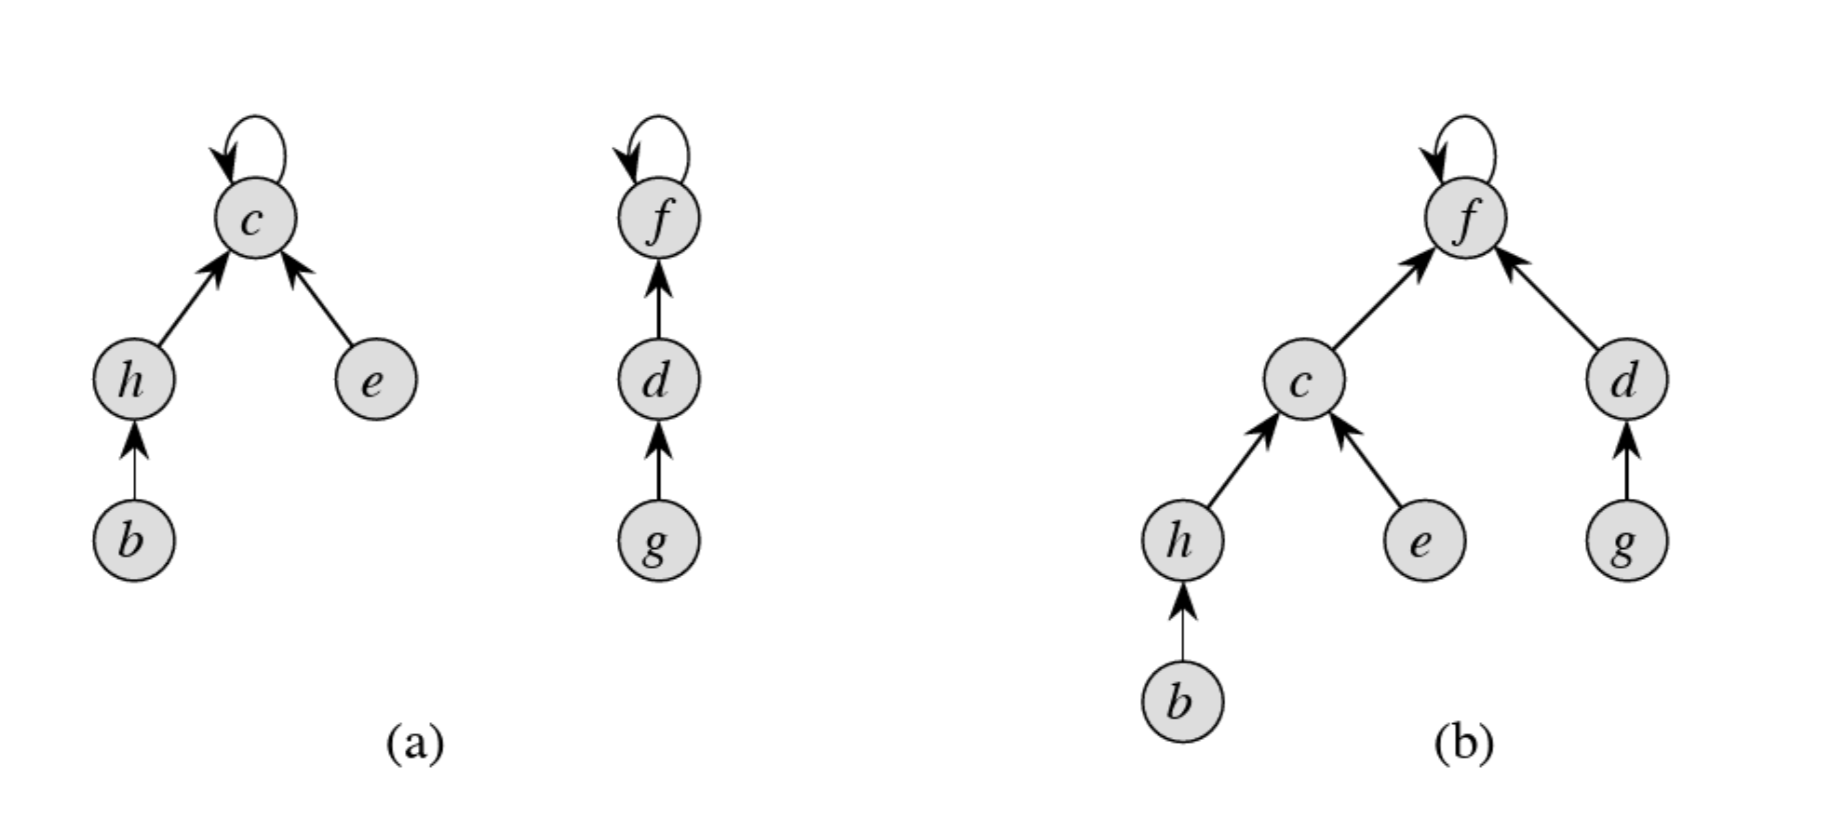
\includegraphics[width=\linewidth]{images/disjointsetforest.png}
            \caption{Before: $S_1$ and $S_2$; After $S_1 := S_1 \cup S_2$}
            \label{fig:disjointsetforest}
        \end{figure}

        On this implementation, this may be no faster than the linked-list implementation (we may just create a chain of $n$ nodes). However using \textbf{union by rank} and \textbf{path compression}, we can get an almost linear runtime. \\ \\
        
        For each node we maintain a \textit{rank}, an upper bound on the height of the tree. We make the root with the smaller rank point to the root with the larger rank during a $UNION$ operation, incrementing the rank of the top root if the two ranks are the same. \\ \\
        

        \begin{figure}[H]
            \centering
            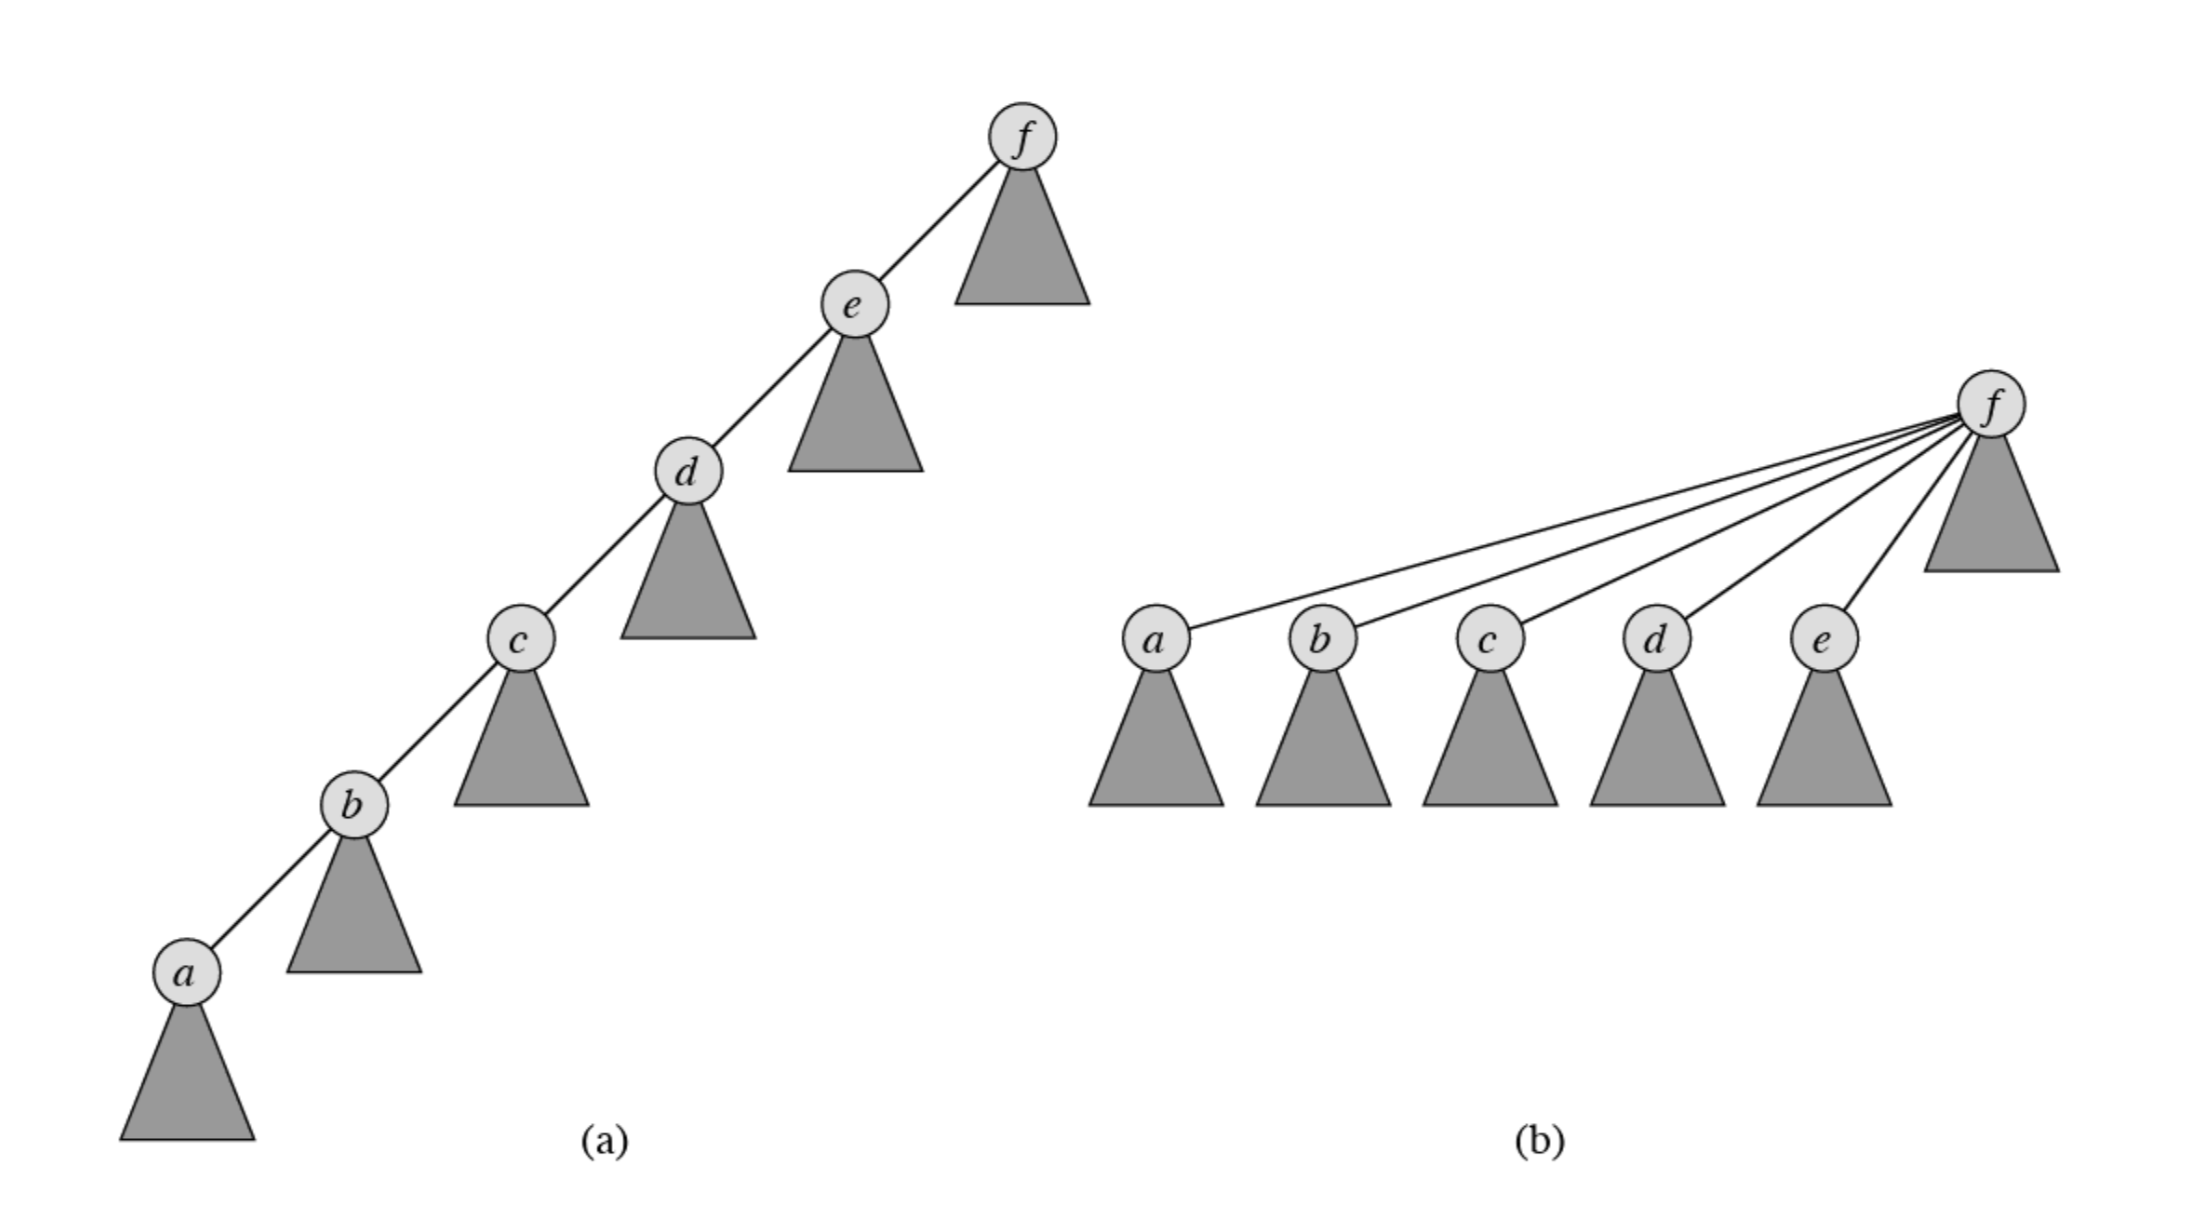
\includegraphics[width=\linewidth]{images/pathcompression.png}
            \caption{Before and after a FIND-SET operation}
            \label{fig:pathcompression}
        \end{figure}
        
        During any invocation of FIND-SET$(x)$, all nodes found whilst traversing up the tree then have their parents redirected to the root (the representative). In this way we flatten long chains in trees. \\ \\
        Using both these heuristics, the runtime is now $O(m \ log^* n)$

\section{Binary Trees}

    \subsection{Binary Search Trees}

    A binary search tree is a dynamic data structure composed of nodes. Each nose has a value, $val[x]$, a left and right child, $left[x]$ and $right[x]$, and a parent, $p[x]$. If there is no child, then we set the respective pointer to $NIL$. \\ \\
    Binary search trees have the BST Property, for every node $x$ in $T$,
    \begin{itemize}
        \item $val[x]$ is greater than all values in the left subtree of $x$
        \item $val[x]$ is less than all values in the right subtree of $x$. 
    \end{itemize} 
    
    \noindent BSTs support several operations:
    \begin{itemize}
        \item INSERT$(T, z)$ - Inserts node $z$ in $T$, time = $O(tree height)$
        \item DELETE$(x)$ - Deletes the node $x$ from its tree. 
            \begin{itemize}
                \item If $x$ has no children, then this is immediate
                \item If $x$ has one child, then we promote this child in place of $x$
                \item If $x$ has two children, find the SUCCESSOR of $x$, $y$. Swap $x$ and $y$, and then delete $x$
            \end{itemize} time = $O(tree height)$
        \item SEARCH$(T,v)$ - Returns $x$ such that $val[x] - v$, if there is such a node, NIL otherwise, time = $O(tree height)$
        \item MIN$(T)$ - Returns $x with$ minimum $val[x]$, time = $O(tree height)$
        \item MAX$(T)$ - Returns $x with$ maximum $val[x]$, time = $O(tree height)$
        \item PREDECESSOR - Returns $y$ such that $y$ has the largest such value smaller than $val[x]$, time = $O(tree height)$
        \item SUCCESSOR$(x)$ - Returns $y$ such that $y$ has the smallest such value greater than $val[x]$, time = $O(tree height)$
    \end{itemize}

    A binary tree is balanced if its height is $O(log \ n)$, hence all operations on a binary tree take time $O(log \ n)$. 

    \subsection{Rotations}

    Rotations can be used to transform one BST into another. They can be performed in $O(1)$ time. Note that rotations also preserve the BST property. 

    \begin{figure}[H]
        \centering
        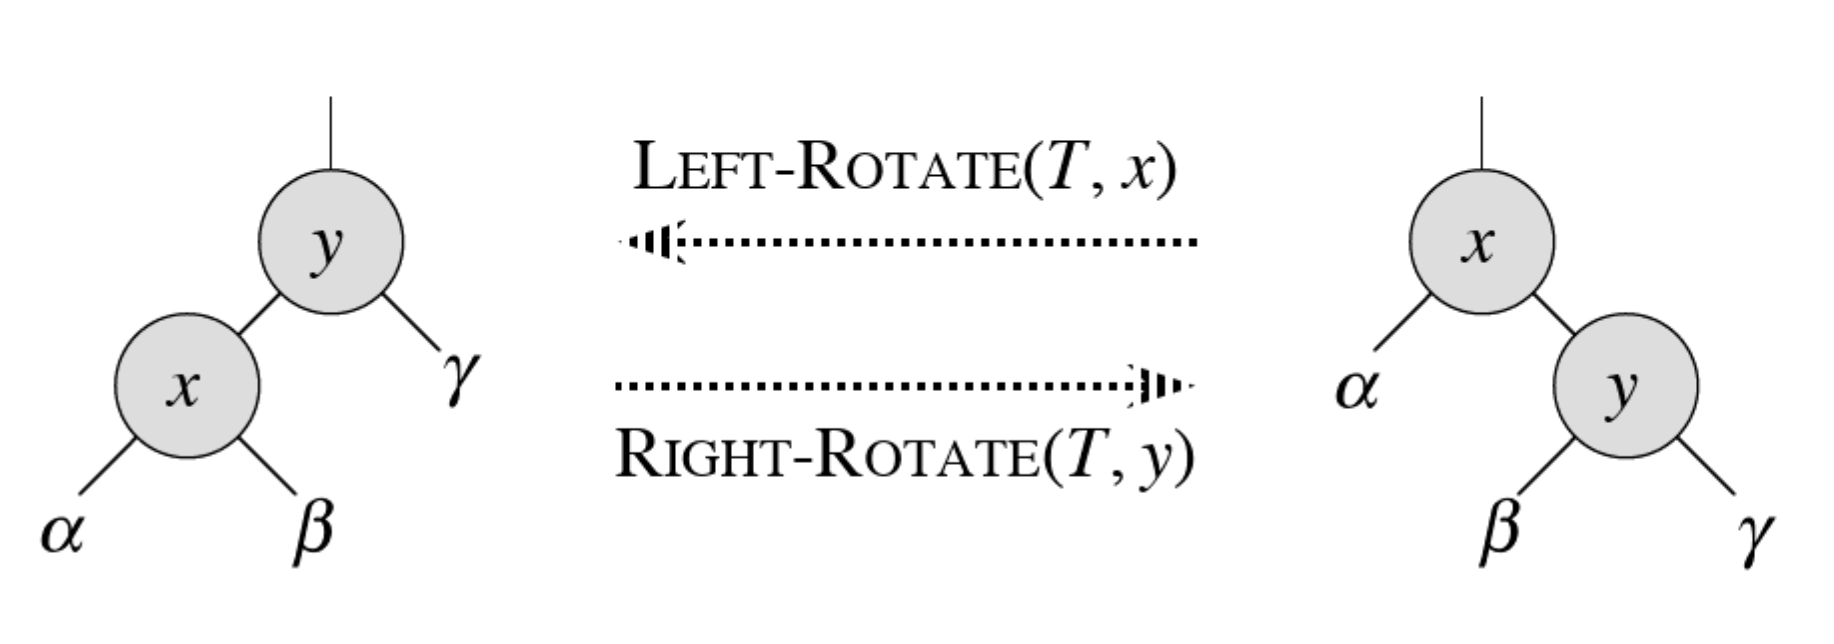
\includegraphics[width=\linewidth]{images/rotate.png}
        \caption{Left and Right rotations}
        \label{fig:rotate}
    \end{figure}
    
    \subsection{Red-Black Trees}

        Red-Black trees are BSTs that also satisfy the following properties:

        \begin{enumerate}
            \item Every node is either red or black
            \item The root is black
            \item Every leaf (NIL) is black
            \item If a node is red, then both its children are black
            \item For each node all simple paths from the node to descendant leaves contain the same number of black nodes. We call this number the \textbf{black height} of $x$
        \end{enumerate}

        \begin{thm}
            A red-black tree $T$ with $n$ items has height $ 2 \ log(n+1)$
        \end{thm}

        This can be proven be showing that :
        \begin{itemize}
            \item height$(T) \leq 2 bh(T)$
                \begin{itemize}
                    \item Consider an arbitrary path $P$ from root to leaf
                    \item The number of red nodes in $P$ $\leq$ the number of black nodes in $P$ 
                \end{itemize}
            \item $bh(T) \leq log \ (n+1)$
                \begin{itemize}
                    \item This can be shown by induction on the height of the tee
                    \item We can also collapse every red node to its black parent, since every value-bearing node has $\geq 2$ children and the height of the collapsed tree is $bh(T)$, then we know that $2^{bh(T)} \leq \# \text{ of } NILs \text{ in collapsed tree} = n + 1$
                \end{itemize}
        \end{itemize}

        Hence BST operations on a red-black tree take $O(log \ n)$ time. \\ \\
        \subsubsection{Insertions}
            To insert into a red-black tree, we insert a red node into the tree. This ensures that the number of black nodes on a path is maintained. Note that this may mean that there are some red-red violations between the inserted node and its parent. To resolve this, we use rotations to move this violation upwards until it reaches the root. \\ \\
            There are three cases when resolving red-red violations:
            \begin{description}
            \item[Case 1] Uncle[x] is red
                \begin{itemize}
                    \item In this case, we recolour the parent and uncle of $x$ black, and the grandparent $red$. 
                    \item Note if the grandparent is the root, then we keep the root colour black.
                    \item We also need to recurse on the grandparent of $x$ as we may have created a new red-red violation
                \end{itemize}
            \item[Case 2] Uncle[x] is black, the triple $(x, p[x], p[p[x]])$ is not aligned
                \begin{itemize}
                    \item In this case, we rotate $x$ with its parent
                    \item This turns the case into case 3, we recurse on the old parent of $x$
                \end{itemize}
            \item[Case 3] Uncle[x] is black, the triple $(x, p[x], p[p[x]])$ is aligned
                \begin{itemize}
                    \item In this case, we rotate the parent of $x$ with the grandparent of $x$. 
                    \item We colour the old grandparent of $x$ red, and the old parent of $x$, black. 
                \end{itemize}
            \end{description}

            \begin{figure}
                \centering
                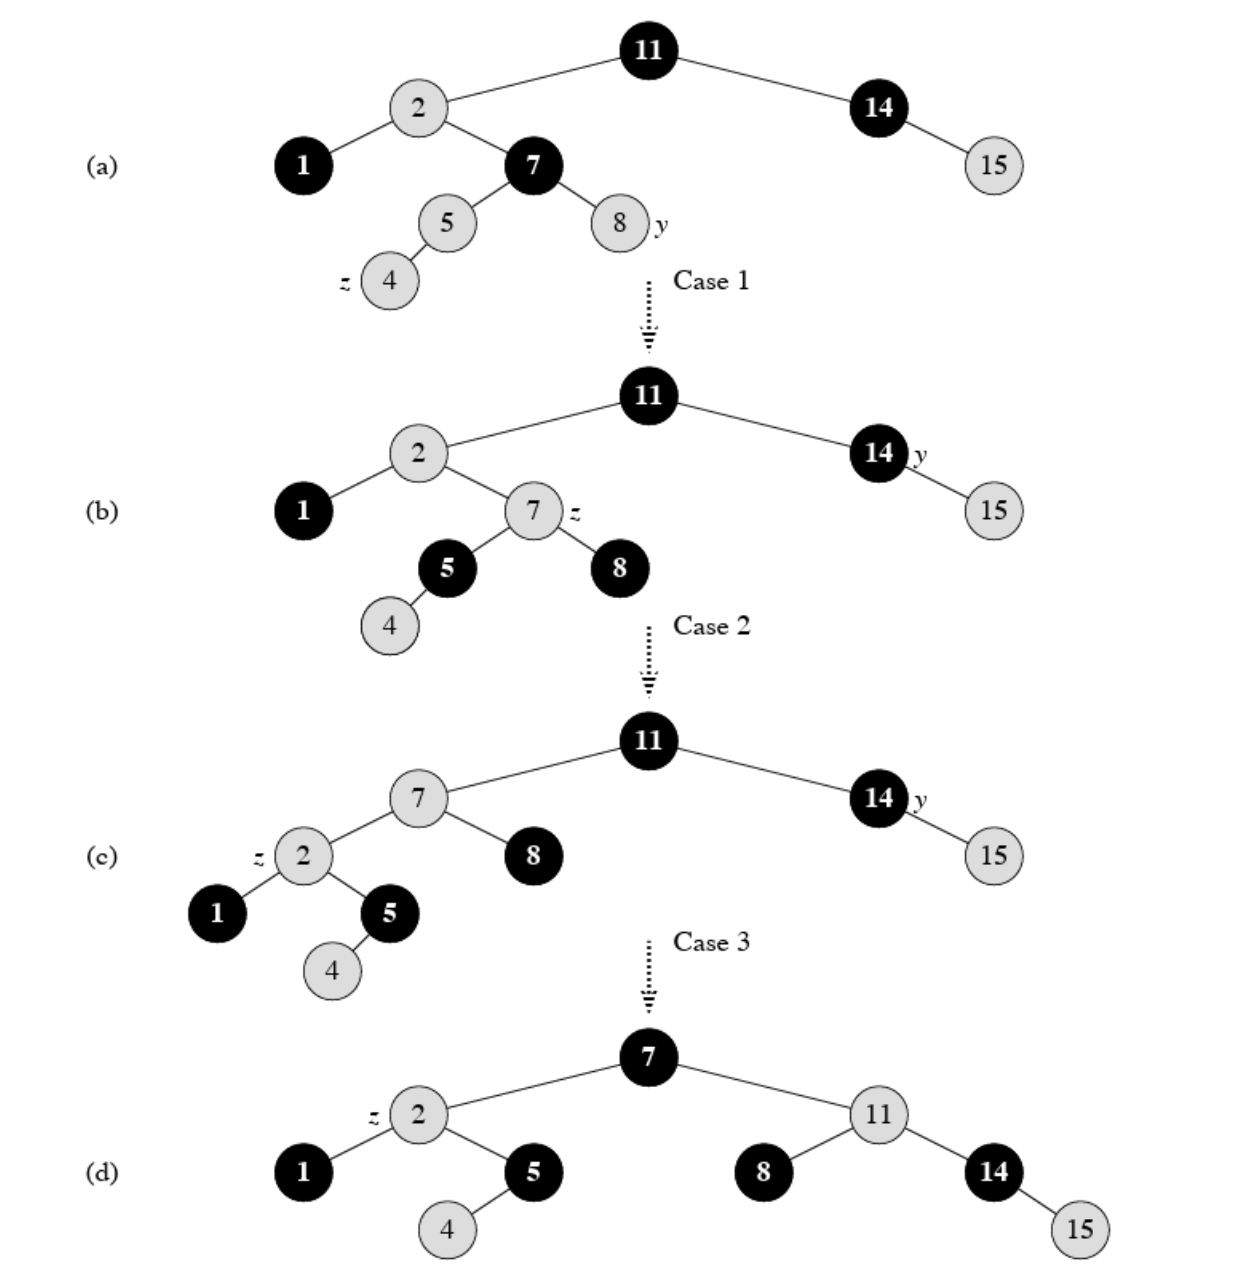
\includegraphics[width=\linewidth]{images/redblack.png}
                \caption{All three cases of a resolving red-red violations}
                \label{fig:redblack}
            \end{figure}

            Since case 3 occurs at most one, case 2 occurs at most once, and case 1 occurs at most the height of the tree, it takes $O(log \ n)$ time to resolve red-red violations. 
    \subsection{Statically Optimal Trees}

    Let $S = \{ x_1, x_2, \ldots, x_n \}$ be the set of values in a BST tree. In a sequence of $m$ searches, $x_i$ is accessed $mp_i$ times (so $p_1 + \ldots + p_n = 1$). The lookup cost of $x_i$ is $1 + \text{depth}(x_i)$. A \textbf{statically optimal binary search tree} is the tree that has the minimum aggregate lookup cost among all BSTs on $n$ items. \\ \\
    There is an $O(n^2)$ time dynamic programming algorithm for constructing statically optimal BSTs, and an $O(n \ log \ n)$ time algorithm that acheives a lookup cost of at most $\frac{3}{2}$ times the optimal lookup cost. Note that both of these methods require that the access probabilities are known in advance. 
    \subsection{Splay Trees}

    Splay trees are self-adjusting BSTs, that adapt to the access sequence. They do not store any additional data, and support BST operations in $O(log \ n)$ amortised time. The principle of splay trees is that when we access an item $x$, we move it to the root of the tree via rotations. In the long run, frequently accessed items are closer to the top of the tree, so that they don't take as much time to find. \\ \\

    \noindent The splay procedure, SPLAY$(T,x)$ is as follows, recursing up until x is at the root
    \begin{itemize}
        \item If $x$ has a parent $y$ but no grandparent
            \begin{itemize}
                \item rotate $x$ with $y$
            \end{itemize}
        \item If the triple $(x, p[x] = y, p[p[x]] = z)$ is aligned (zig-zig)
            \begin{itemize}
                \item rotate $y$ with $z$
                \item rotate $x$ with $y$
            \end{itemize}
        \item If the triple $(x, p[x] = y, p[p[x]] = z)$ is not aligned (zig-zag)
            \begin{itemize}
                \item rotate $x$ with $y$
                \item rotate $x$ with $z$
            \end{itemize}
    \end{itemize}

    \begin{figure}
            \centering
            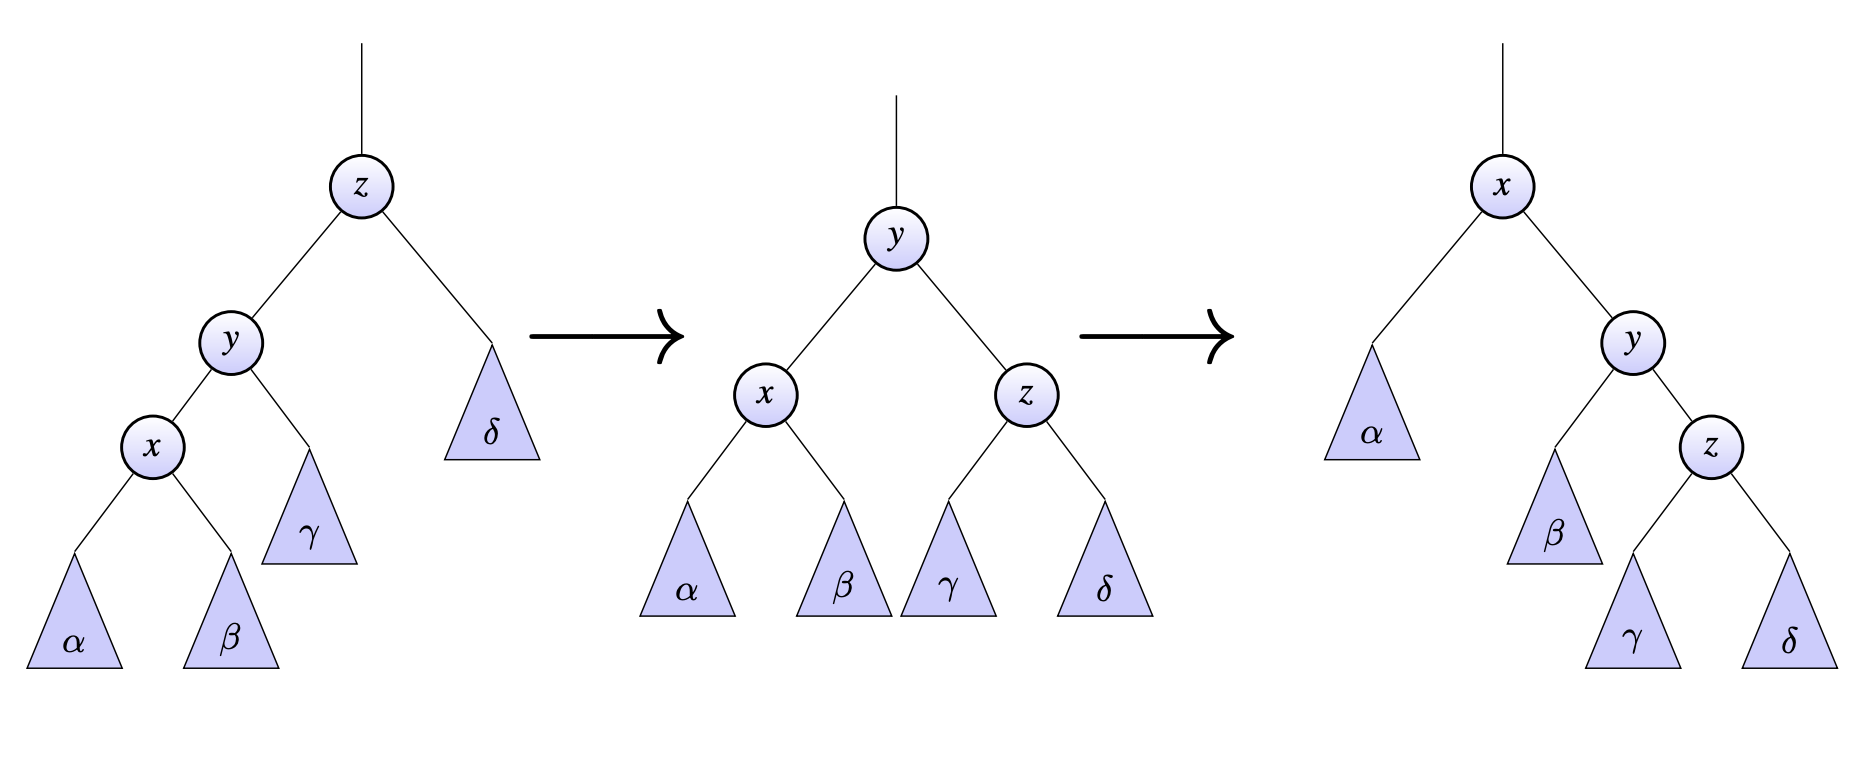
\includegraphics[width=\linewidth]{images/zigzig.png}
            \caption{Zig-zig}
            \label{fig:zigzig}
    \end{figure}

    \begin{figure}
            \centering
            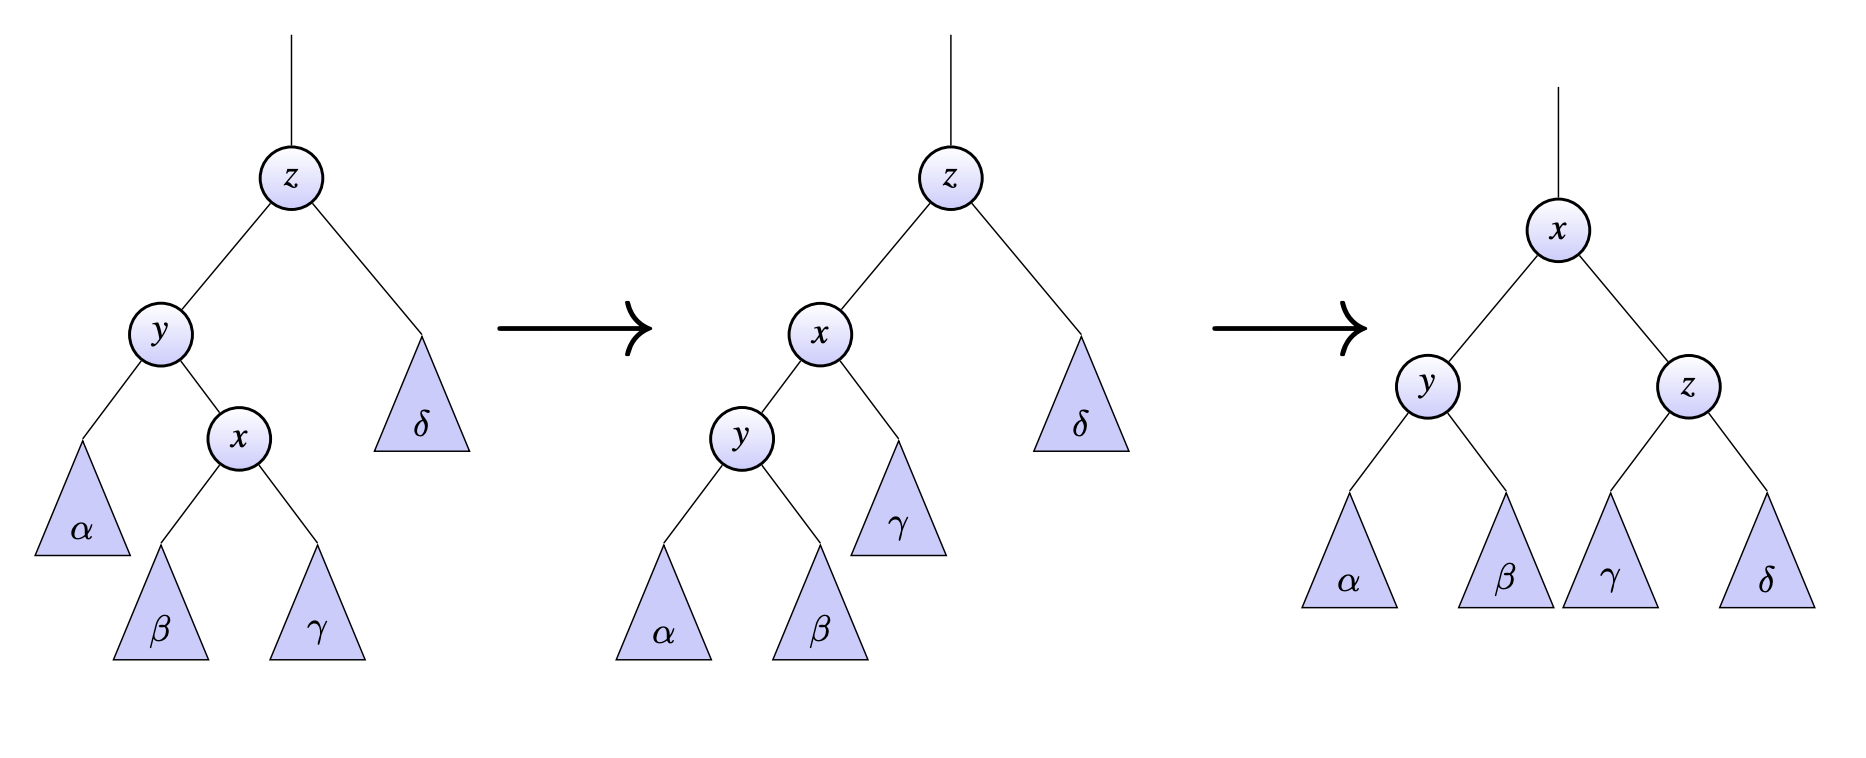
\includegraphics[width=\linewidth]{images/zigzag.png}
            \caption{Zig-zag}
            \label{fig:zigzag}
    \end{figure}

    We may also need to modify BST operations to support splaying a tree:
    \begin{itemize}
        \item SEARCH$(T,x)$ - Perform SPLAY$(T, x)$
        \item INSERT$(T,x)$ - Insert x into T as usual and then perform SPLAY$(T, x)$
        \item DELETE$(T,x)$ - Perform SPLAY$(T, x)$, then remove x from the root. This splits the tree into $T_{< x}$ and $T_{> x}$. Find $w = max(T_{< x})$, perform SPLAY$(T_{< x}, w)$, and then join $T_{> x}$ on $w$, which we can do as $w$ has no right child. 
    \end{itemize}

    The amortised cost of SPLAY is $O log \ n$. This analysis can be performed by the potential function method. It can then be shown that for $n$ INSERTS and $m$ SEARCH/DELETE operations, the total cost is $O((m + n) log n)$. 
    
\section{Flow Networks}

    \begin{defn}
        A \textbf{flow network} is a directed graph $G = (V,E)$ in which each edge $(u, v) \in E$ has a non-negative capacity $c(u,v) \geq 0$. Furthermore if $(u,v) \in E$, then $(v, u) \notin E$. We distinguish two nodes in G, the \textbf{source} $s$ and the \textbf{sink} $t$, such that for each vertex $v \in V$, the flwo network contains a path $s \rightsquigarrow v \rightsquigarrow t$
    \end{defn}

    \begin{defn}
        A \textbf{flow} in G is a real-valued function $f : V \times V \to \mathbb{R}$ that satisfies

        \begin{description}
            \item[Capacity Constraint] For all $u, v \in V$, we require \[0 \leq f(u,v) \leq c(u,v)\]
            \item[Flow Constraint] For all $u \in V - \{ s,t \} $ we require \[ \sum_{v \in V} f(u,v) = \sum_{v \in V}f(u,v) \]
        \end{description}
        Note that when $(u,v) \notin E$, then $f(u,v) = 0$
    \end{defn}

    \noindent The \textbf{value} of $f$ is defined as
    \[ |f| = \sum_{e \text{ out of } s}f(e) \]
    
    \begin{figure}
            \centering
            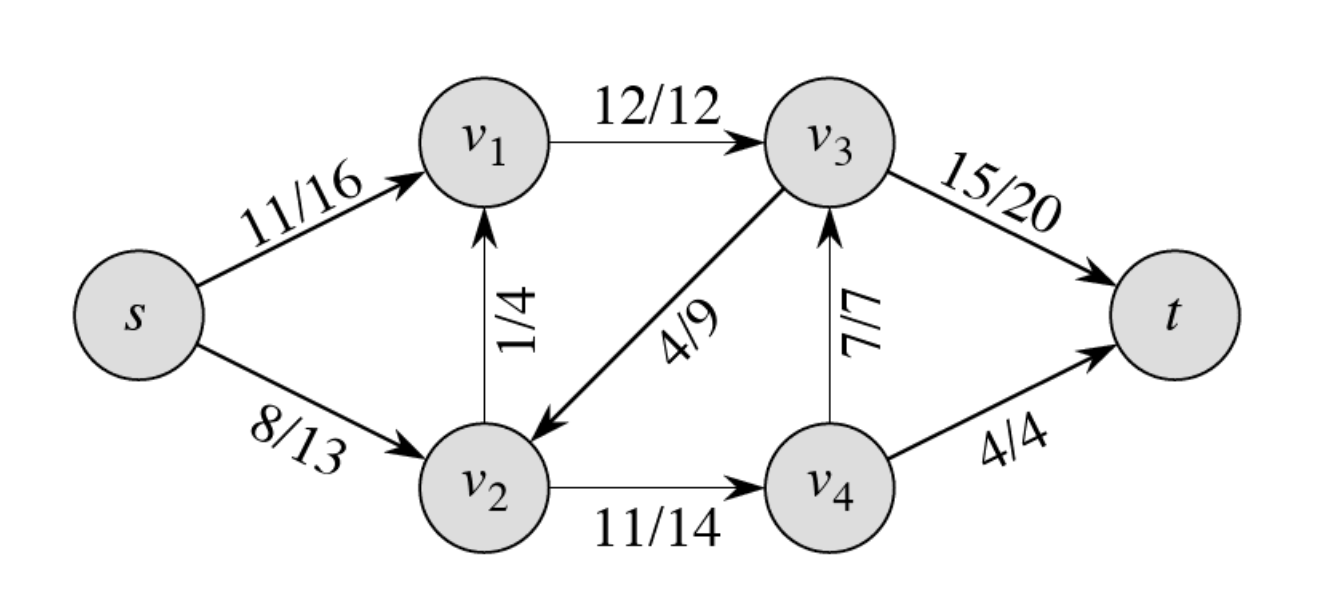
\includegraphics[width=\linewidth]{images/flownetwork.png}
            \caption{Example Flow Network}
            \label{fig:flownetwork}
    \end{figure}

    \subsection{Minimum Cut}
        \begin{defn}
            An \textbf{s-t cut} is a partition of $V$ into $A, B$ such that $s \in A$ and $t \in B$. 
        \end{defn}
        The \textbf{capacity} of an s-t cut $(A,B)$ is defined as 
        \[ \text{cap}(A,B) = \sum_{e \text{ out of } A} c(e) \]
        The minimum cut of a flow network is an s-t cut with minimum capacity. \\ \\
        \begin{defn}
            \textbf{Weak Duality} If $(G, s, t, c)$ is a flow network, then
            \[ \text{value of max flow} \leq \text{capacity of min s-t cut} \]
            i.e. for any flow $f$ and any s-t cut $(A, B)$
            \[ |f| \leq \text{cap}(A,B) \]
        \end{defn}
        \noindent We can prove weak duality by observing that due to flow conservation, 
        \[ |f| = \sum_{e \text{ out of } A} f(e) -  \sum_{e \text{ into } A} f(e)\]
        and hence
        \begin{align*}
            |f| &\leq  \sum_{e \text{ out of } A} f(e) \\  
            &\leq  \sum_{e \text{ out of } A} c(e)
            \\ &= c(A,B)
        \end{align*}
        As a corollary result, if $f$ satisfies $|f| = \text{cap}(A,B)$, then f is a maximum flow. Hence to certify $f$ is a maximum flow, it suffices to find a corresponding s-t cut. 
        \subsection{Residual Graphs}

        Given a flow network $G$ and a flow $f$, the residual network $G_f$ consists of edges with capacities that represent how we can change the flow on edges of G. An edge of the flow network can admit an amount of additional flow equal to the edge's capacity minus the flow on that edge. Since a network may also decrease the flow on particular edges, we need backward edges on $G_f$ with a capacity equal to the flow on the original edges, i.e. to build $G_f$,
        \begin{itemize}
            \item $G_f$ has the same edges as $G$
            \item For each $e = (u,v)$ with flow $f(e)$ and capacity $c(e)$
            \begin{itemize}
                \item If $f(e) < c(e)$ - add forward edge $(u,v)$ with capacity $c_f((u,v)) = c(e) - f(e)$
                \item If $f(e) > 0$ - add backward edge $(v,u)$ with capacity $c_f((v,u)) = f(e)$
            \end{itemize}
        \end{itemize}

    \subsection{Augmenting Paths}
        \begin{defn}
            Given a flow network $G = (V, E)$ and a flow $f$, an \textbf{augmenting path} $p$ is a simple path from $s$ to $t$ in the residual network $G_f$. By definition of the residual network, we can increase the flow on an edge in $G$, $(u,v)$ by up to $c_f(u,v)$
        \end{defn}

        We can also define the bottleneck capacity, $b_P$, of an augmenting path and a flow $f$ in $G$ as the the minimum residual capacity $c_f(e)$ over $e \in P$. We can therefore augment $f$ by $b_P$ units of flow. \\ \\
        \noindent AUGMENT$(f, P)$ : construct flow $f'$ on $G$
        For each $e \in E$:
        \begin{itemize}
            \item if $e \in P$ set $f'(e) = f_e + b_P$
            \item if $rev(e) \in P$ set $f'(e) = f_e - b_P$
            \item otherwise, set $f'(e) = f(e)$
        \end{itemize}
        If $f$ is a flow in G and $P$ is an augmenting path in $G_f$, then
        \begin{itemize}
            \item $f' = $ AUGMENT$(f, P)$ is a valid flow in $G$
            \item $|f'| = |f| + b_P$
        \end{itemize}
        Hence calling AUGMENT on a graph always increases the flow. 
        
        \begin{thm}
            The \textbf{Max-Flow Min-Cut} theorem states that if $f$ is a flow in $G$, with source $s$ and sink $t$, then the following are equivalent:
            \begin{enumerate}
                \item $f$ is a maximum flow in $G$
                \item The residual network $G_f$ has no augmenting paths
                \item $|f| = \text{cap}(S,T)$ for some cut $(S,T)$ of $G$
            \end{enumerate}
        \end{thm}

        We can prove $(1) \to (2)$ by observing that if the residual graph did have an augmenting path $P$, then we can increase the flow in $G$ by $b_P$, meaning that $f$ can't be a maximum flow. \\ \\
        Suppose $G_f$ has no augmenting paths, meaning we can split $V$ into the nodes reachable from $s$, $A$ and all other nodes, $B$.  Clearly $s \in A$ and $t \in B$. Consider a pair of vertices $u \in A$, $v \in B$. If $(u,v) \in E$, then we must have $f(u,v) = c(u,v)$ as otherwise $(u,v) \in E_f$, meaning $v$ would be reachable from $s$. Similarly, if $(v,u) \in E$, $f(v,u) = 0$, as otherwise $c_f(u,v) = f(v, u)$ would be positive, meaning $(u,v) \in E_f$, and hence $v$ would be reachable from $s$. If neither $(u,v)$ nor $(v,u)$ is in $E$, then $f(u,v) = f(v,u) = 0$. Hence
        \begin{align*}
            f(A,B) &= \sum_{u \in A} \sum_{v \in B} f(u,v) - \sum_{v \in B} \sum_{u \in A} f(v,u) \\ 
            &= \sum_{u \in A} \sum_{v \in B} c(u,v) - \sum_{v \in B} \sum_{u \in A} 0 \\
            &= \text{cap}(A,B)
        \end{align*}

        Since $(A,B)$ is a cut of the network, $|f| = f(A,B) = c(A,B)$ thus proving $(2) \to (3)$. \\ \\
        We can finally prove $(3) \to (1)$ by weak duality. 
    
    \subsection{Ford-Fulkerson}

        FORD-FULKERSON(G,s,t,c)
        \begin{algorithmic}[1]
            \State{Set $f(e) = 0$ for all $e \in E$}
            \State{$G_f$ := residual graph of $G$ wrt $f$}
            \While{there exists s-t path $P$ in $G_f$}
                \State{$f := $ AUGMENT$(f,P)$}
                \State{Update $G_f$}
            \EndWhile
        \end{algorithmic}
        We also know that the Ford-Fulkerson algorithm returns a maximum flow as upon termination $G_f$ has no s-t path, and is therefore disconnected. This means that we can split $V$ into $(A, B)$, where $A$ are all the vertices reachable from $s$. $(A, B)$ is a cut of $G$ with $cap(A, B) = |f|$, which by weak duality implies $f$ is a max-flow .
        \\ \\
        We can only be certain that this algorithm terminates when the capacities are integers. Since the flow increases by at least $1$ at each iteration, the total time is $O(m|f^*|)$, where $m$ is the number of edges in G, $|f^*|$ is the value of the maximum flow. \\ \\
        In order to improve the runtime of the Ford-Fulkerson Algorithm, we want to find the largest bottleneck capacity each time. A good heuristic is the capacity-scaling algorithm. This algorithm uses a parameter $\Delta$ which starts large and decreases by a factor of 2. We only consider a subgraph of $G_f$ that contains edges with a capacity $\geq \Delta$. In this way, we increase the flow by at least half the max bottleneck capacity every while loop. \\ \\
        CAPACITY-SCALING$(G,s,t,c)$
        \begin{algorithmic}[1]
            \State{Set $f(e) = 0$ for all $e \in E$, $C = \max_{e \in E} c(e) $}
            \State{$\Delta := $ largest power of 2 less than or equal to C}
            \While{$\Delta \geq 1$}
                \State{$G_f$ := residual graph of $G$ wrt $f$}
                \While{there exists s-t path $P$ in $G_f$}
                    \State{$f := $ AUGMENT$(f,P)$}
                    \State{Update $G_f$}
                \EndWhile
                \State{$\Delta := \Delta / 2$}
            \EndWhile
            \State{return $f$}
        \end{algorithmic}
        Since every path in $G_f(\Delta)$ is a path in $G_f$, and $G_f(\Delta) = G_f$, we know that CAPACITY-SCALING returns a maximum flow. \\ \\
        Let $C =$ maximum capacity edge in G. The outer loop of the algorithm runs $1 + log \ C$ times.
        \begin{lemma}
            After the end of a $\Delta$-scaling phase, $|f^*| \leq |f| + m \Delta$, where $f^*$ is the maximum flow.
        
        \end{lemma}
        
         This is true because after the $\Delta$-scaling phase, there is no s-t path in $G_f(\Delta)$, and we can therefore partition $V$ into $(A, B)$, where $A$ is all the vertices reachable from $s$, $B = V \setminus A$. Hence
        \begin{itemize}
            \item For each $(u,v) \in E$ with $u \in A$, $v \in B$
            \begin{itemize}
                \item $c(e) < f(e) + \Delta$
            \end{itemize}
            \item For each $(u,v) \in E$ with $u \in B$, $v \in A$
            \begin{itemize}
                \item $f(e) < \Delta$
            \end{itemize}
        \end{itemize}
        as otherwise there would be an $s-t$ path in $G_f(\Delta)$. Therefore
        \begin{align*}
            |f| &= \sum_{e \text{ out of } A} f(e) - \sum_{e \text{ into} A} f(e)\\ 
            &\geq \sum_{e \text{ out of } A} (c(e) - \Delta) - \sum_{e \text{ into} A} \Delta \\ 
            &\geq \text{cap}(A,B) - \Delta m \\
            &\geq |f^*| - \Delta m
        \end{align*}
        Hence by this lemma, we can see that the inner loop is executed $\leq 2m$ times. This is because after the previous execution of the inner loop, by the lemma we have $|f^*| \leq |f| + 2 \Delta m$ and each augmentation in a $\Delta$-phase increases $f$ by at least $\Delta$. \\ \\ 
        Since the outer loop takes $O(1 + log \ C)$, the inner loop takes $O(m)$ and it takes $O(m)$ time to find an s-t path, the total runtime is $O(m^2 (1 + log \ C))$
    \subsection{Edmonds-Karp}
        EDMONDS-KARP$(G,s,t,c)$
        \begin{algorithmic}[1]
            \State{Set $f(e) = 0$ for all $e \in E$}
            \State{$G_f := $ residual graph wrt $f$}
            \While{There exists s-t path in $G_f$}
                \State{$P := $ s-t path with fewest edges}
                \State{$f := $ AUGMENT$(f, P)$}
                \State{Update $G_f$}
            \EndWhile
            \State{Return $f$}
        \end{algorithmic}

        The idea behind that Edmonds-Karp Algorithm is that edges don't become bottlenecks too often. \\ \\
        We can show that the runtime of this algorithm is $O(nm^2)$ by examining two claims, (not proven here). Consider the $i$th time that the loop is executed. Let $f_i$ be the flow at the beginning of the loop, $G_i$ the residual graph wrt $f_i$ and $d_i(u,v)$ be the distance between $u$ and $v$ in $G_i$ 
        \begin{description}
            \item[Claim 1] For any vertex $v \in V$, $d_i(s,v)$ is non-decreasing with $i$, i.e.
            \[ d_1(s,v) \leq d_2(s,v) \leq \ldots \]
            \item[Claim 2] If $e$ is the bottleneck edge at time $i$, it will not be used in an augmenting path again until $d_i(s,t)$ increases
        \end{description}
        Using these two claims, we can see that the distance between $s$ and $t$ can increase at most $n$ times. For each value $d = distance(s,t)$ in $G_f$, an edge becomes a bottleneck at most once, so there are at most $m$ augmentations for $d \in [1, n]$. Since the time taken to find $P$ uses $BFS$, which is $O(m)$, the total time taken is $O(nm^2)$. 
        
    \subsection{Bipartite Matchings}
        \begin{defn}
            Given an undirected graph $G=(V,E)$ a \textbf{matching} is a subset of edges $M \subseteq E$ such that for all $v \in V$, at most one edge of $M$ is incident on $v$. If an edge is incident on $v$ in a matching $M$, then this vertex is \textbf{matched}, otherwise it is \textbf{unmatched}. A \textbf{maximum matching} is a matching of maximum cardinality. 
        \end{defn}

        \begin{figure}
            \centering
            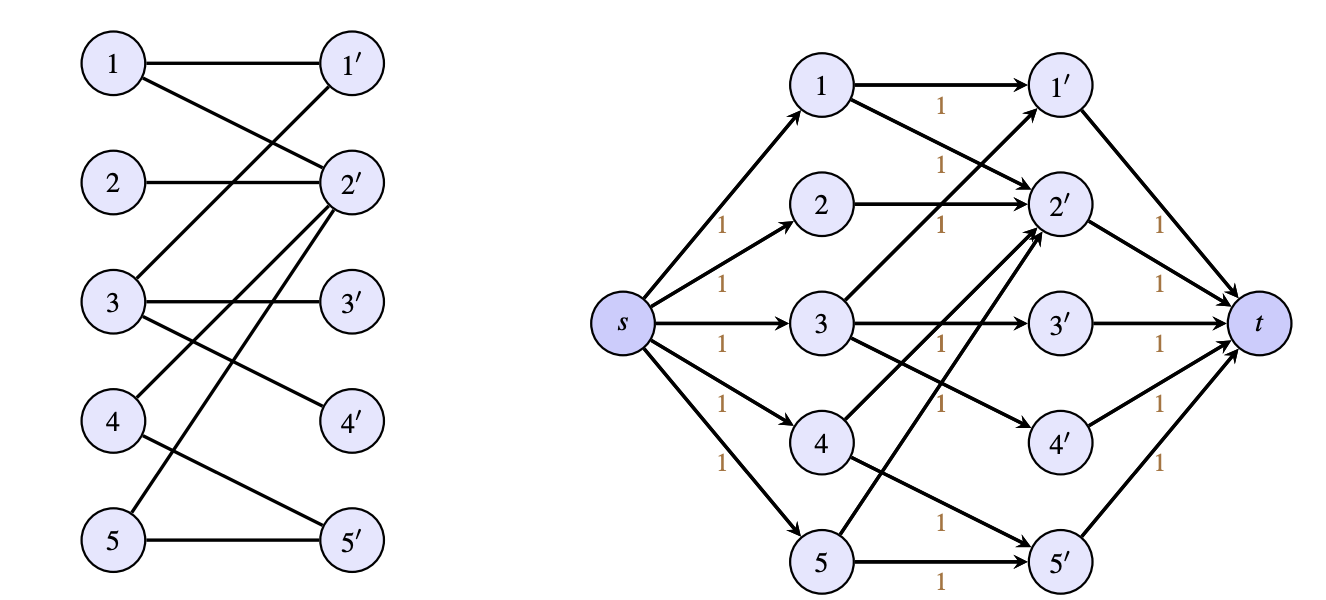
\includegraphics[width=\linewidth]{images/bipartite.png}
            \caption{Constructing a flow network from a bipartite graph}
            \label{fig:bipartite}
        \end{figure}

        Given an instance $G = (L \cup R, E)$ of a \textbf{bipartite} matching problem, we can create an instance $G' = (V',E')$ of MAXFLOW by adding a source node $s$ that connects to every node in $L$, a sink node that is connected to every node in $R$, and by setting all edge capacities to 1. G has a maximal matching equal to $k$ iff the max flow on $G'$ is equal to k. \\ \\
        A matching is called \textbf{perfect} if every vertex is matched. We can use this algorithm to find the perfect matching, if it exists. A certificate for when a graph $G$ does not have a perfect matching is when there is a set of vertices in $L$ that has a number greater than that of the set of neighbouring vertices, i.e. there is some $S \in L$ such that 
        \[ |N(S)| \leq |S| \]
        However, the converse statement also holds
        \begin{thm}[Hall's Theorem]
            A bipartite graph $G = (L \cup R, E)$ has a perfect matching iff for every set $S \subseteq L$ it holds that $|N(S)| \geq |S|$
        \end{thm}
        To prove the converse direction, suppose that for every $S \subseteq L$, $|N(S)| \geq |S|$. Consider the constructed flow network G', with an arbitrary s-t cut $(A, B)$. Let $A_L = A \cap L$, $A_R = |A \cap R|$. Hence
        \begin{align*}
            \text{cap}(A, B) &= \sum_{e \text{ out of } A} \\ 
            &\geq |L \setminus A_L| + |N(A_L) \setminus A_R| + |A_R| \\
            &\geq |L| - |A_L| + |N(A_L)| - |A_R| + |A_R| \\ 
            &\geq |L| - |A_L| + |A_L| - |A_R| + |A_R|  \tag{by assumption} \\ 
            &= |L| \\
            &= n
        \end{align*}
        By the max-flow min-cut theorem, since the minimum capacity is at least $n$, then the max flow is $n$, hence $G'$ has a maximum flow, and so $G$ has a perfect matching. 
        
    \subsection{Circulations}

        \begin{defn}
            Given a directed graph $G = (V, E)$, capacity bounds $c : E \to \mathbb{Z}^+$ and a demand function $d : V \to \mathbb{Z}$ the \textbf{circulation problem} is to find a \textbf{circulation} $f : E \to \mathbb{R}^+$ such that for each edge $e \in E$
            \[ 0 \leq f(e) \leq c(e) \tag{Capacity Constraint}\]
            and for each $v \in V$
            \[ \sum_{e \text{ into } v} f(e) - \sum_{e \text{ out of } v} f(e)= d(v) 
 \tag{Flow Conservation} \]
        \end{defn}
        \noindent Note that for any circulation, by flow conservation, we must have that 
        \[ \sum_{v \ : \ d(v) > 0} d(v) = \sum_{v \ : \ d(v) < 0} |d(v)|  \]
        Given a circulation instance $(G,c,d)$, we can construct a flow network $(G', s, t, c)$ by
        \begin{itemize}
            \item Adding a source $s$ and sink $t$
            \item For each $v$ with $d(v) < 0$, add edge $(s,v)$ with capacity $-d(v)$
            \item For each $v$ with $d(v) > 0$, add edge $(v,t)$ with capacity $d(v)$
        \end{itemize}

        \begin{figure}
            \centering
            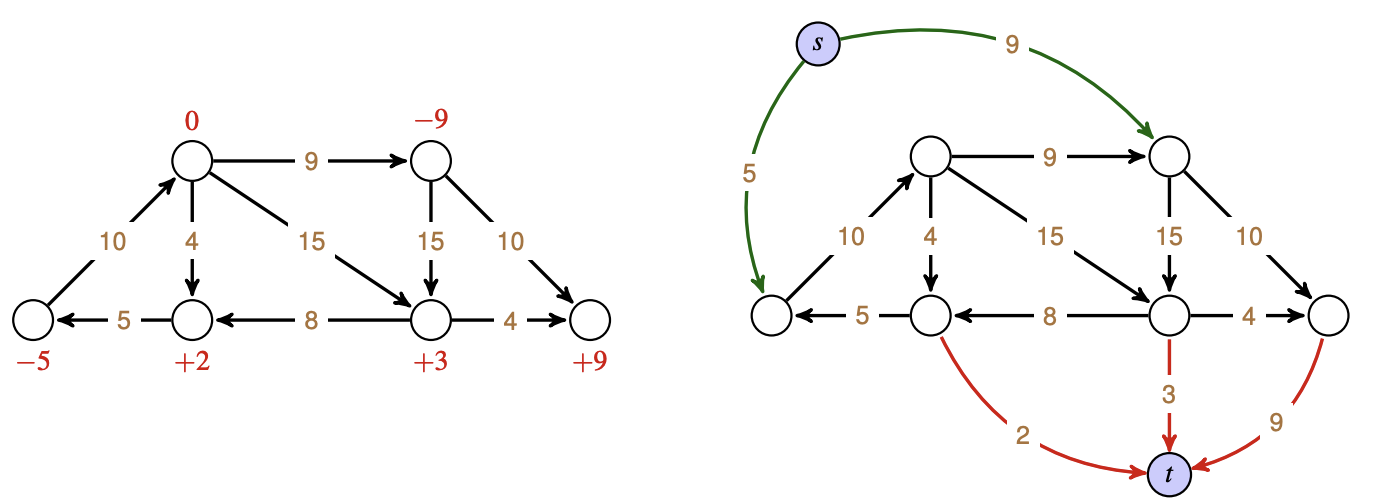
\includegraphics[width=\linewidth]{images/circulation.png}
            \caption{Constructing a flow network from a circulation instance}
            \label{fig:circulation}
        \end{figure}
        
        We can see that $G$ has a circulation iff $G'$ has max flow equal to 
        \[ D = \sum_{v \ : \ d(v) > 0} d(v) =  \sum_{v \ : \ d(v) < 0} |d(v)| \]
        In this way, the sink and source nodes mimic the demand functions of the circulation. \\ \\
        Suppose instead that in addition t capacity bounds, we also have s lower bounds for the circulation, $l : E \to \mathbb{Z}^+$. We can still format this as a network flow problem. We do this by constructing the circulation as before, and for each edge $e = (u,v)$ with $l(e) > 0$
        \begin{itemize}
            \item $d'(u) := d(u) + l(e)$
            \item $d'(v) := d'(v) - l(e)$
            \item $c(e) := c(e) - l(e)$
            \item $l(e) := 0$
        \end{itemize}
        Meaning that we act as if these lower bounds are being satisfied, with the capacities and the demand of $v$ being lowered and the demand of $u$ being raised. 

        \begin{figure}
            \centering
            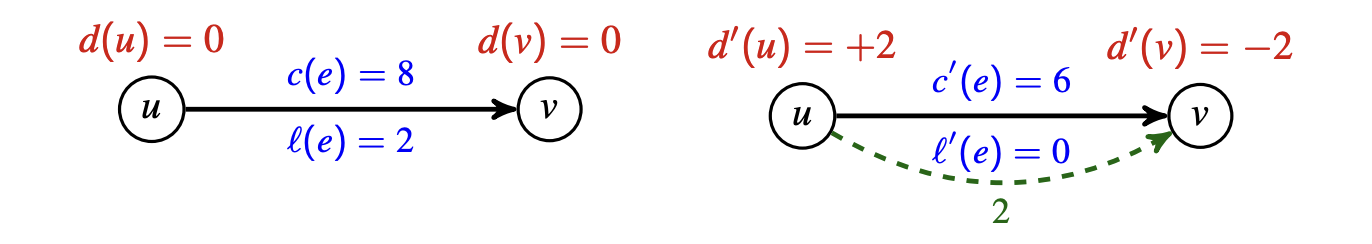
\includegraphics[width=\linewidth]{images/lowerbound.png}
            \caption{Removing lower bound constraints}
            \label{fig:lowerbound}
        \end{figure}

\section{Minimum Cost Perfect Matchings}

    Given an undirected bipartite graph $G = (X \cup Y, E)$, and a cost function $c : E \to \mathbb{R}^+$, how can we find a perfect matching $M$ such that $c(M)$ is minimised? This algorithm can't be achieved using network flows, as network flows encode \textbf{constraints} for problems, however this problem deals with \textbf{preferences}. \\ \\
    The structure of the algorithm assumes at any stage there is a matching of size $i$. We then find an augmenting path that will produce a matching of size $i + 1$. We use the cheapest augmenting path at each stage so that the larger matching will have the minimum cost. \\ \\
    Recall the construction of the residual graph used for finding augmenting paths, let $M$ be a matching. We also add the source $s$ and the sink $t$ nodes. We add edges $(s,x)$ for all nodes $x \in X$ that are unmatched and edges $(y,t)$ for all nodes $y \in Y$ that are unmatched. This residual graph is denoted by $G_M$. Note that wrt to a flow $f$,
    \begin{itemize}
        \item If $(x, y) \in M$, then $(y,x) \in G_M$ (as we can reduce this flow to 0)
        \item If $(x, y) \notin M$, then $(x,y) \in G_M$ (as we can increase this flow). 
    \end{itemize}

    \begin{figure}
        \centering
        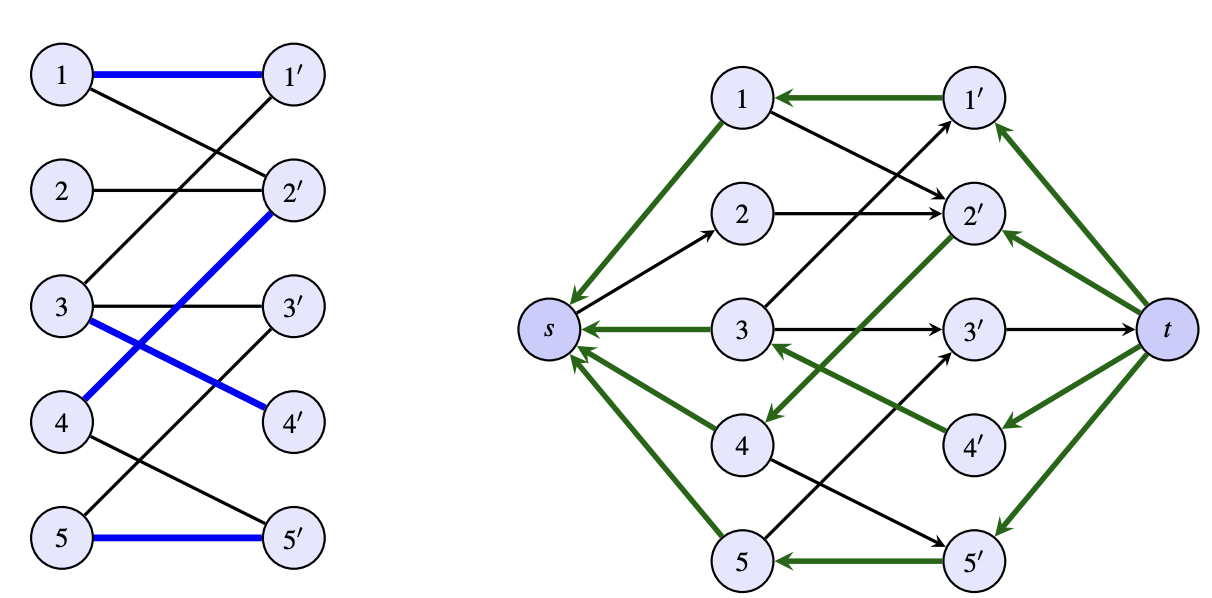
\includegraphics[width=\linewidth]{images/mincostresidual.png}
        \caption{Residual graph of a matching}
        \label{fig:mincostresidual}
    \end{figure}
    
    Note that any augmenting path in $G_M$ starts at $s$ and alternates between matched and unmatched edges. When we start at $s$, we go to an unmatched node. We must then use an unmatched edge, as the only edges that go from $X$ to $Y$ in $G_M$ are those where $(x,y) \notin M$. Likewise, we must then use an matched edge to go from $Y$ to $X$. Finally we go from an unmatched vertex to t. \begin{figure}
        \centering
        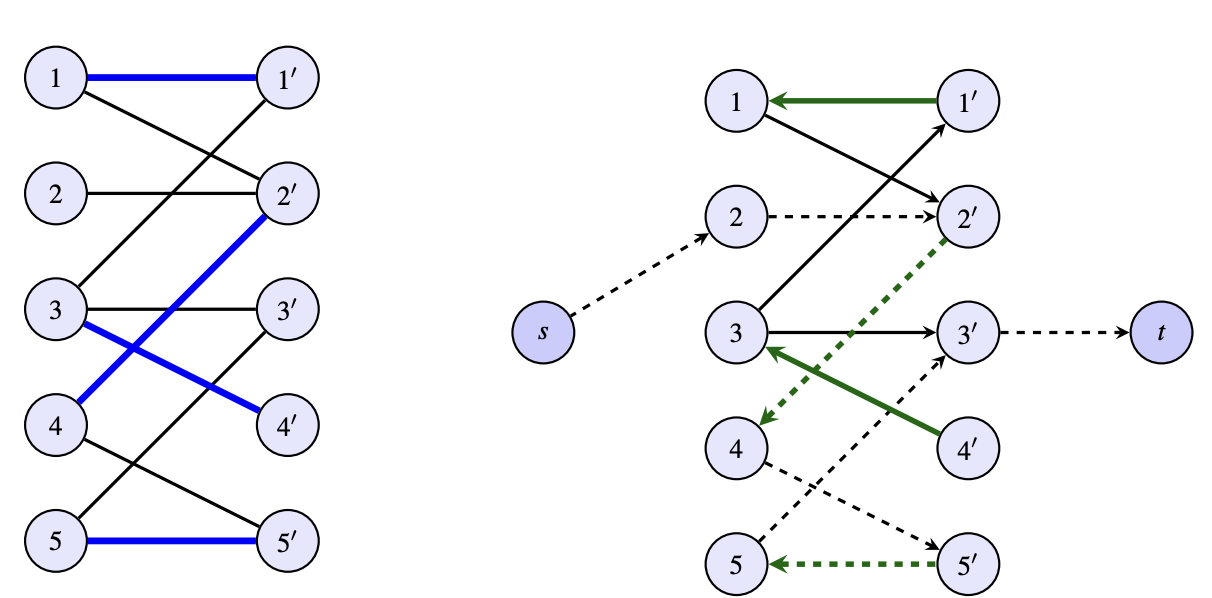
\includegraphics[width=\linewidth]{images/alternatingpath.png}
        \caption{An augmenting path alternates between unmatched and matching nodes}
        \label{fig:alternatingdiff}
    \end{figure}
    Hence when we take the symmetric difference of any matching $M$ and an augmenting path $P$, we must result in a matching $M' = M \oplus P$ that has one more matching than $M$. This is because we can think of the action of using an edge from $X$ to $Y$ as being equivalent to including it in the new matching $M'$, and using an edge from $Y$ to $X$ as being equivalent to discounting it from $M'$. Since we go from $X$ to $Y$ once more than we go from $Y$ to $X$, we must have increased the number of edges by 1. 
    \begin{figure}
        \centering
        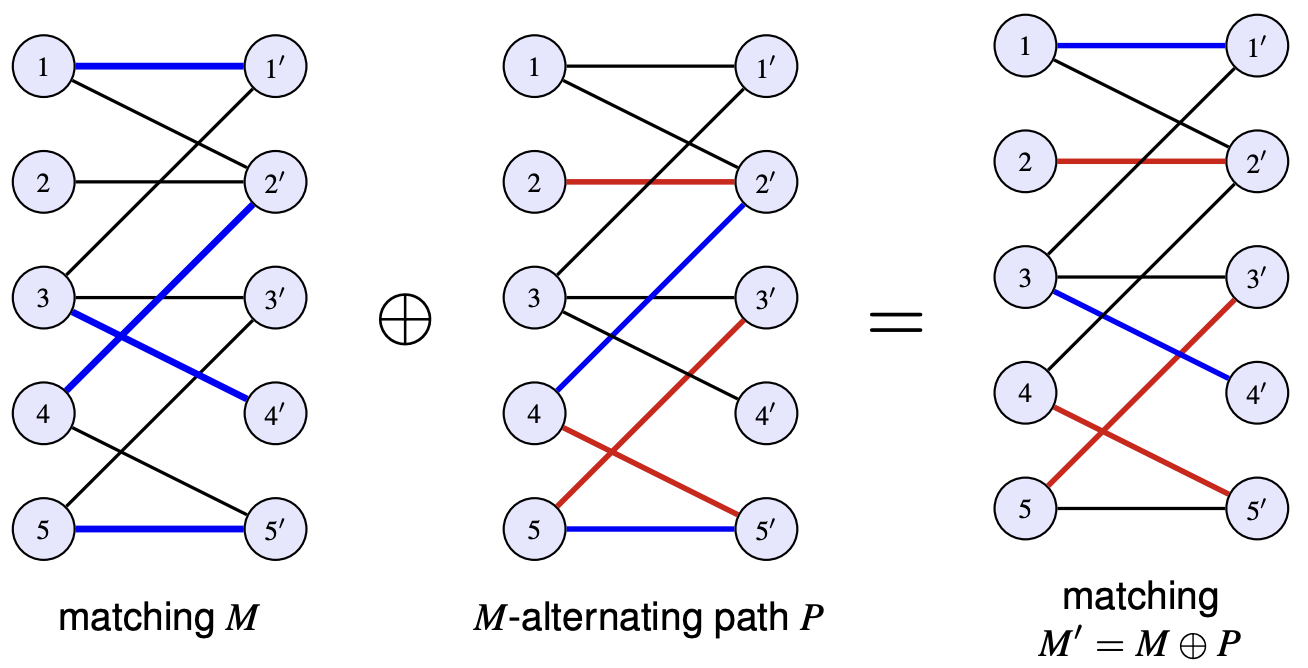
\includegraphics[width=\linewidth]{images/augmentingdiff.png}
        \caption{Constructing a new matching of a larger size}
        \label{fig:augmentingdiff}
    \end{figure}

    The cost of this alternating path is hence each $c(x,y)$ as we add edges $(x,y)$ to $M$ minus each $c(y,x)$ as we remove these edges from $M$. We also define the cost of each edge in $M$ to reflect this:
    \begin{itemize}
        \item If $(x, y) \in M$ then cost of $(x,y)$ in $G_M$ is $-c(x,y)$
        \item If $(x, y) \notin M$ then cost of $(x,y)$ in $G_M$ is $c(x,y)$
        \item All edges from $s$ or into $t$ have cost $0$
    \end{itemize}
    Hence on this definition, 
    \[ c(M') = c(M) + c(P) \]
    
    We can see that this algorithm may fail to produce a well-defined output when there exist negative cycles in the residual graph $G_M$. 
    %TODO finish notes about negative cycles

\section{Linear Programming}

    \begin{defn}
         A \textbf{linear program} is an optimisation problem over real-valued variables. We maximise or minimise a linear \textbf{objective} function subject to linear \textbf{constraints}. Note that these constraints are $\leq, \geq, =$, but not $>, <$
    \end{defn}
    \begin{alignat*}{2}
        \text{maximise} &\quad 2x + 5y  && \\
        \text{subject to} &\quad 3x + 5y &&\leq 15 \\
        &\quad x + y &&\leq 4 \\
        &\quad -x - 10y &&\geq -20 \\
        &\quad x,y &&\geq 0
    \end{alignat*}

    A linear program is \textbf{feasible} if there is a solution satisfying all the constraints. It is \textbf{bounded} if the optimal value is finite. 
    \begin{thm}[Fundamental Theorem of Linear Programming]
        For an LP, exactly one holds:
        \begin{itemize}
            \item The LP is infeasible
            \item The LP is feasible but unbounded
            \item The LP is bounded, feasible and there is a solution that achieves OPT, the optimum value of the objective function. 
        \end{itemize}
    \end{thm}

    To solve LPs, we can consider the feasible set, all the points that satisfy the constraints. The optimal value must then be at an intersection point, hence if we find the values of the objective function at these extreme points, we can then find the optimal value for the objective function. 

    \subsection{Dual Linear Programs}

        \begin{defn}
            The \textbf{dual} of a linear program (called the \textbf{primal}) is a closely related LP whose feasible and optimal solutions provide information about the primal LP.
        \end{defn}
        For example, if the primal LP is a maximisation problem, then the dual gives upper bounds on the optimal value (and similarly lower bounds on minimisation problems).

        As we have seen, a general LP consists of $n$ real variable, an objective function and several constraints of the form $\geq, \leq =$. In order to write the dual of a linear program, we must first write the linear program in standard max form. This consists of
        \begin{itemize}
            \item Replacing all min functions with max functions
            \begin{itemize}
                \item min $x_1 - 2x_2 $ becomes 
                \item  max $-x_1 + 2x_2$
            \end{itemize}
            \item Replacing all $=$ constraints with $\leq and \geq$ constraints
            \begin{itemize}
                \item $x + y = 1 $ becomes 
                \item $ x + y \geq 1$, $x + y \leq 1$
            \end{itemize}
            \item Replacing all $\geq$ constraints with $\leq$ constraints
            \begin{itemize}
                \item $x + y \geq 1 $ becomes 
                \item $ -x-y \leq -1$
            \end{itemize}
            \item Making all variables non-negative by writing them as the difference between a non-negative variable and a non-positive variable
            \begin{itemize}
                \item $x \leq 1 $ becomes 
                \item $ x^+ - x^- \leq 1$ and $x^+, x^- \geq 0$
            \end{itemize}
        \end{itemize}

        We now have a primal LP of the form

        \begin{alignat*}{2}
        \text{maximise} &\quad c_1 x_1 + c_2 x_2 + \ldots + c_n x_n  && \\
        \text{subject to} &\quad a_{11}x_1 + a_{12}x_2 + \ldots + a_{1n}x_n &&\leq b_1 \\
        &\quad a_{21}x_1 + a_{22}x_2 + \ldots + a_{2n}x_n &&\leq b_2 \\
        &    &&  \vdots \\ 
        &\quad a_{m1}x_1 + a_{m2}x_2 + \ldots + a_{mn}x_n &&\leq b_n \\
        &\quad x_1,x_2,\ldots,x_n &&\geq 0 \\
        \end{alignat*}

        We then construct the dual by 
        \begin{itemize}
            \item Multiplying the $i$th constraint with $y_i \geq 0$
            \begin{itemize}
                \item $y_i( \sum^n_{j=1} a_{ij}x_j ) \leq b_i y_i$
            \end{itemize}
            \item Summing these new inequalities to obtain $L \leq $ BOUND
            \begin{itemize}
                \item BOUND $= \sum^m_{i=1} b_i y_i $
                \item $L = \sum^m_{i=1} y_i(\sum^n_{j=1} a_{ij}x_j) = \sum^n_{j=1} x_j \sum^m_{i=1} a_{ij} y_i$
            \end{itemize}
            \item Ensuring that the objective function $\leq L$ by imposing constraints on each $y_i$
            \begin{itemize}
                \item $c_j \leq \sum^m_{i=1} a_{ij}y_i$ for each $j = 1, \ldots, n$
            \end{itemize}
            \item Optimising each $y_i$ to find the minimum value of BOUND. 
            \begin{itemize}
                \item min $ \sum^m_{i=1} b_i y_i $
            \end{itemize}
        \end{itemize}

        Hence the dual LP can now be written as 

        \begin{alignat*}{2}
        \text{minimise} &\quad b_1 y_1 + b_2 y_2 + \ldots + b_m y_m  && \\
        \text{subject to} &\quad a_{11}y_1 + a_{21}y_2 + \ldots + a_{m1}y_m &&\geq c_1 \\
        &\quad a_{12}y_1 + a_{22}y_2 + \ldots + a_{m2}y_m &&\geq c_2 \\
        &    &&  \vdots \\ 
        &\quad a_{1n}x_1 + a_{2n}x_2 + \ldots + a_{mn}y_m &&\geq c_n \\
        &\quad y_1,y_2,\ldots,y_m &&\geq 0 \\
        \end{alignat*}

        Note that the $b_i$'s and the $c_i$'s have switched, the rows of the $a_{ij}$'s have become columns and instead of $n$ variables and $m$ constraints, there are $m$ variables and $n$ constraints. This allows us to capture (standard) LPs in terms of matrices. The primal LP has now become
\begin{alignat*}{2}
        \text{maximise} &\quad \mathbf{c}^T \mathbf{x}  && \\
        \text{subject to} &\quad A \mathbf{x} &&\leq \mathbf{b} \\
        &\quad \mathbf{x} &&\geq 0 \\
        \end{alignat*}
        
        And the dual now becomes:
        \begin{alignat*}{2}
        \text{minimise} &\quad \mathbf{b}^T \mathbf{y}  && \\
        \text{subject to} &\quad A^T \mathbf{y} &&\geq \mathbf{c} \\
        &\quad \mathbf{y} &&\geq 0 \\
        \end{alignat*}

        \begin{thm}[Weak LP Duality]
            Let $\mathbf{x}$ be in the feasible region of the primal LP and $\mathbf{y}$ be in the feasible region of the dual LP. Then
            \[ \mathbf{c}^T \mathbf{x} \leq \mathbf{b}^T \mathbf{y} \]
        \end{thm}

        We can see this is true as
        \begin{align*}
            \mathbf{c}^T \mathbf{x} &= \mathbf{x}^T \mathbf{c} \\
            &\leq \mathbf{x}^T A^T \mathbf{y} \\
            &= (A \mathbf{x})^T \mathbf{y} \\
            &\leq \mathbf{b}^T \mathbf{y}
        \end{align*}

        Hence if $\mathbf{c}^T \mathbf{x} = \mathbf{b}^T \mathbf{y}$, then these objective functions must have reached their optimum. 
        \begin{thm}[Strong LP Duality]
            Suppose either of the primal or dual LP is bounded and feasible. Then both of them are, and the optimum value of the primal is equal to the optimal value of the dual
        \end{thm}
    \subsection{Solving LPs}
        To solve the LP 
        \begin{alignat*}{2}
        \text{maximise} &\quad \mathbf{c}^T \mathbf{x}  && \\
        \text{subject to} &\quad A \mathbf{x} &&\leq \mathbf{b} \\
        &\quad \mathbf{x} &&\geq 0 \\
        \end{alignat*}
        \begin{itemize}
            \item Enumerate all vertices of the polyhedron $P = \{ \mathbf{x} \in \mathbb{R}^n \ | \ A \mathbf{x} \leq \mathbf{b} \}$
            \item Find the vertex with the maximum value of the objective function
            \item Check that the LP is bounded
            \begin{itemize}
                \item Use the dual LP  and check that it is feasible
            \end{itemize}
        \end{itemize}

        %TODO Simplex
    \subsection{Applications of LPs}
        \subsubsection{Max Flows}
            We can formulate flow networks as LPs, as we are trying to maximise the flow on each edge whilst being constrained by the capacities on each edge. \\ \\ 
            Given a flow network $G = (V,E,s,t)$ and a capacity function $c : E \to \mathbb{Z}^+$ create the LP:
            
            \begin{alignat*}{5}
            \text{maximise} &\quad \sum_{e \text{ out of } s}f_e && \\
            \text{subject to} &\quad f_e &&\geq 0  \tag{for each $e \in E$} \\
            &\quad f_e &&\leq c(e) \tag{for each $e \in E$} \\
            &\quad \sum_{e \text{ out of } v}f_e - \sum_{e \text{ into } v} f_e &&= 0 \\
            \end{alignat*}
            where $f_e$ is the flow on each edge in the network.
        \subsubsection{Circulations}
            We can also formulate circulation, however as this is a feasibility problem instead of an optimisation problem, there is no objective function. However, this may be an issue as we need to find a starting point for the algorithms available to solve LPs. Hence we introduce nonnegative slack variables for the demands at each of the vertices, if the objective function at its minimum manages to be $0$, then there is a circulation.

            \begin{alignat*}{5}
            \text{minimise} &\quad \sum_{v \in V} q_v^+ + q_v^- && \\
            \text{subject to} &\quad l(e) &&\leq f_e  \tag{for each $e \in E$} \\
            &\quad f_e &&\leq c(e)  \tag{for each $e \in E$} \\
            &\quad \sum_{e \text{ out of } v}f_e - \sum_{e \text{ into } v} f_e &&= d(v) + q_v^+ - q_v^- \tag{for each $v \in V$} \\
            &\quad q_v^+, q_v^- \geq 0 \tag{for each $v \in V$}
            \end{alignat*}
            Now to find the initial starting point, we set $f_e = l(e)$ for all $e \in E$. Let $A_v$ be the excess flow for each node, i.e.
            \[ A_v = \sum_{e \text{ into } v} f_e - \sum_{e \text{ out of } v}f_e \]
            If $A_v \geq 0$, set $(q_v^+, q_v^-) = (A_v, 0)$ , otherwise set $(q_v^+, q_v^-) = (0, -A_v)$
        \subsubsection{Min-Cost Circulation}
            We can also formulate min-cost circulations more directly, given $G = (V,E)$ a demand function $d: V \to \mathbb{Z}$, upper and lower capacity bounds $c, l : E \to \mathbb{Z}$ and a cost function $k: E \to \mathbb{Z}$, we can form the LP
            \begin{alignat*}{5}
            \text{minimise} &\quad \sum_{e \in E}k(e)f_e && \\
            \text{subject to} 
            &\quad l(e) &&\leq f_e  \tag{for each $e \in E$} \\
            &\quad f_e &&\leq c(e)  \tag{for each $e \in E$} \\
            &\quad \sum_{e \text{ out of } v}f_e - \sum_{e \text{ into } v} f_e &&= d(v) \tag{for each $v \in V$} \\
            \end{alignat*}
            which will output the minimum cost circulation $\{ f_e \}_{e \in E}$ with min cost $\sum_{e \in E}k(e)f_e$
        \subsubsection{Min-Cost Perfect Matching}
            Given $G = (L \cup R, E)$ and a cost function $c : E \to \mathbb{Z}$, we can form an LP by setting variables $x_e$ to be $1$ if $e$ belongs to the matching, and $0$ otherwise. 
            \begin{alignat*}{5}
            \text{minimise} &\quad \sum_{e \in E}c(e)x_e && \\
            \text{subject to} 
            &\quad \sum_{e \text{ incident to } v} x_e &&= 1  \tag{for each $v \in L \cup R$} \\
            &\quad  x_e &&\in \{0, 1\}  \tag{for each $e \in E$} \\
            \end{alignat*}
            Note that this is an instance of an \textbf{Integer Linear Program} (ILP).
        \subsubsection{Bipartite Perfect Matching}
            Bipartite perfect matching can be given as an ILP, but another solution is to relax the constraints for the LP so that they may be non-integral. \\ \\
            Given $G = (V, E)$ and cost function $c : E \to \mathbb{Z}$ the LP can be written as
            \begin{alignat*}{5}
            \text{minimise} &\quad \sum_{e \in E}c(e)x_e && \\
            \text{subject to} 
            &\quad \sum_{e \text{ incident to } v} x_e &&= 1  \tag{for each $v \in V$} \\
            &\quad  x_e &&\\geq 0 \tag{for each $e \in E$} \\
            \end{alignat*}
            For bipartite graphs this will always give an integer solution (the same is not true for general graphs). \\ \\
            To prove this claim, suppose for the sake of contradiction that $E' = \{e \ | \ 0 < x_e < 1\}$, for an extreme point of the LP, $x$, is non-empty. By the constraints $\sum_{e \text{ incident to } v} x_e = 1$ and $x_e \geq 0$, we know that every vertex v has a degree of either $0$ or $\geq 2$. Hence we know that $G$ has a cycle of even length (as $G$ is bipartite). \\ \\
            Call the edges of the cycle $C = \{e_1, e_2, \ldots, e_{2k} \}$. Define $\epsilon = \text{min} \{x_{e_1}, x_{e_2}, \ldots, x_{e_{2k}}\} $, i.e. the smallest edge in the cycle. We can then define $y$ by
            \[ y_e = 
               \begin{cases}
                    x_{e_i} + \epsilon & \text{if $e = e_i \in C$ and $i$ is even} \\ 
                    x_{e_i} - \epsilon & \text{if $e = e_i \in C$ and $i$ is odd} \\ 
                    x_{e} & \text{otherwise}
               \end{cases}
            \]
            and similarly $z$ by
            \[ z_e = 
               \begin{cases}
                    x_{e_i} - \epsilon & \text{if $e = e_i \in C$ and $i$ is even} \\ 
                    x_{e_i} + \epsilon & \text{if $e = e_i \in C$ and $i$ is odd} \\ 
                    x_{e} & \text{otherwise}
               \end{cases}
            \]
            We have that $x = \frac{1}{2}(y + z)$, but $y$ and $z$ are still feasible, contradicting the assumption that $x$ is an extreme point. 
        \begin{figure}[H]
            \centering
            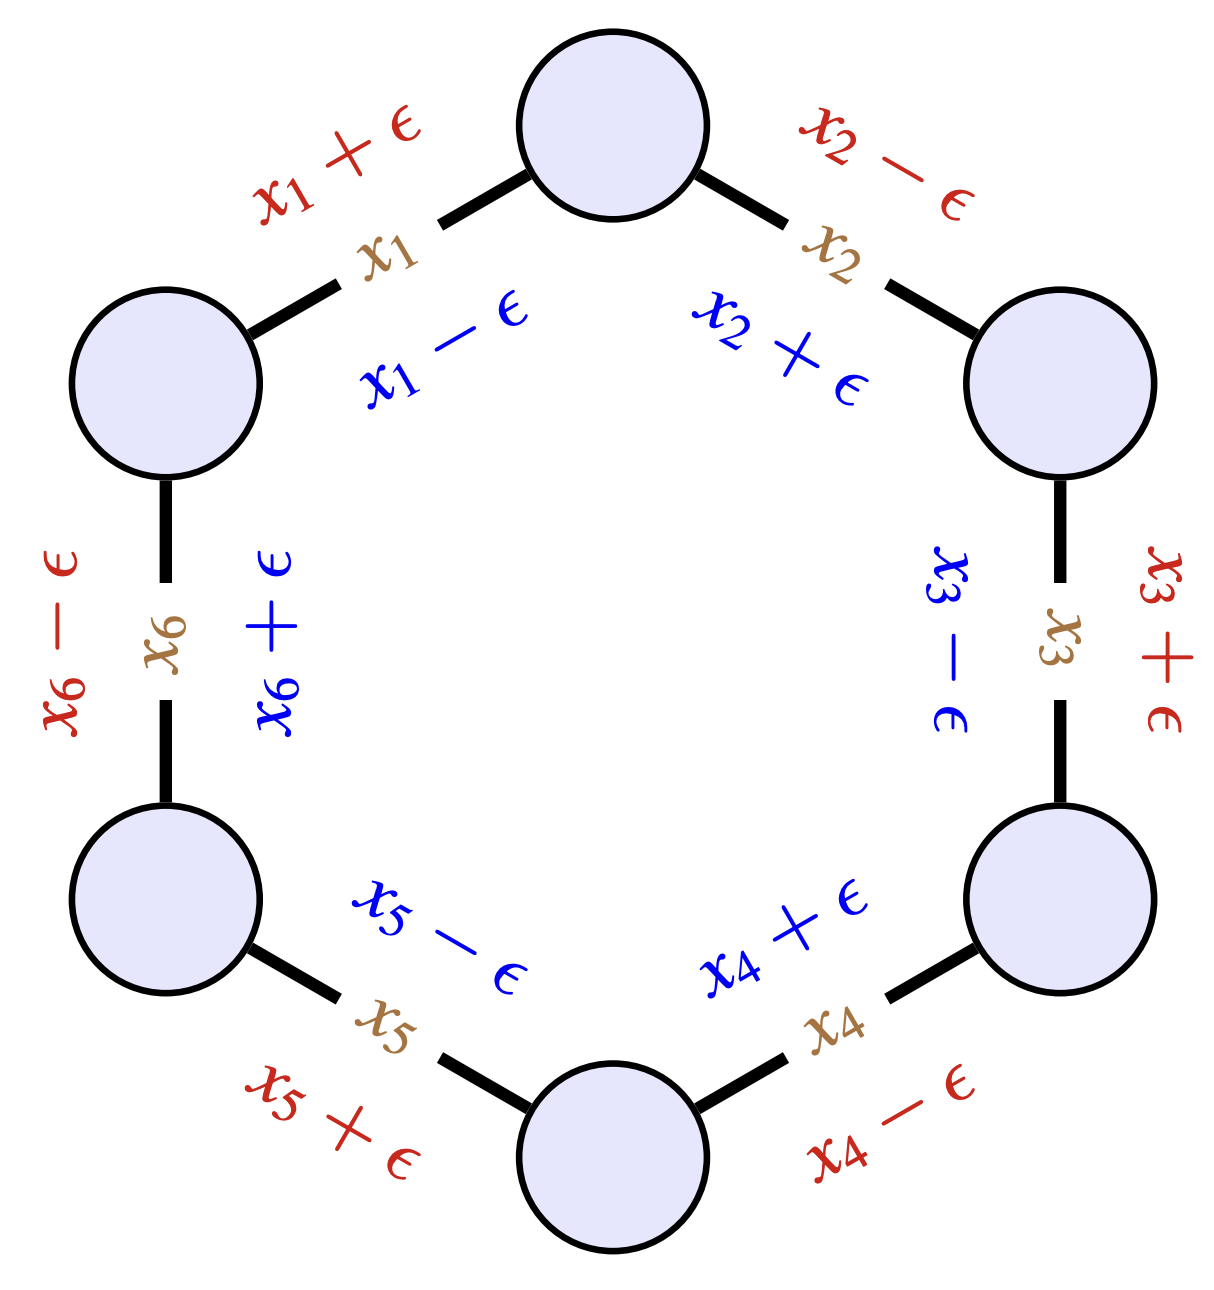
\includegraphics[width=100pt]{images/epsiloncycle.png}
            \caption{We can reduce and increase by $\epsilon$ in both directions without violating the constraint $x_e \geq 0$}
            \label{fig:epsiloncycle}
        \end{figure}
    \subsection{Zero-Sum Games}
        % TODO Write this section
\section{NP Hardness}

    \begin{defn}
        A \textbf{decision problem} is a problem where the answer is either YES or NO
    \end{defn}

    \begin{defn}
        P is the class of decision problems such that for each decision problem $\Pi$ in P there is a polynomial-time algorithm $A$ such that for every instance $x$ of $\Pi$
        \begin{itemize}
            \item if $\Pi(x) = $ YES, then $A(x) =$ YES
            \item if $\Pi(x) = $ NO, then $A(x) = $ NO
        \end{itemize}
    \end{defn}

    \begin{defn}
        NP is the class of decision problems such that for each decision problem $\Pi$ in NP there is a polynomial-time algorithm $A$ and a constant $c > 0$ such that for every instance $x$ of $\Pi$
        \begin{itemize}
            \item if $\Pi(x) = $ YES, then there is a certificate $y$ with $|y| \leq |x|^c$ such that $A(x,y) = $ YES
            \item if $\Pi(x) = $ NO, then for all certificates $y$, $A(x,y) = $ NO
        \end{itemize}
    \end{defn}

    A decision problem in NP can hence be solved by non-deterministically guessing all certificates $y$ with $|y| \leq |x|^c$ and returning whether any of these certificates give $A(x,y) = $ YES. 

    \subsection{Reductions}
        \begin{defn}
            A \textbf{reduction} from a problem $A$ to problem $B$ is a polynomial time algorithm that takes an instance $x$ of $A$ and produces an instance $y = f(x)$ of B such that
            \begin{itemize}
                \item $|y|$ is at most a polynomial in $|x|$
                \item $A(x) = $ YES iff $B(y) = $ YES
            \end{itemize}    
            If $f$ exists, then we write $A \leq B$. 
        \end{defn}
        Intuitively this means that if $B$ can be decided in polynomial-time, then A can also be solved in polynomial-time
        \begin{figure}[H]
            \centering
            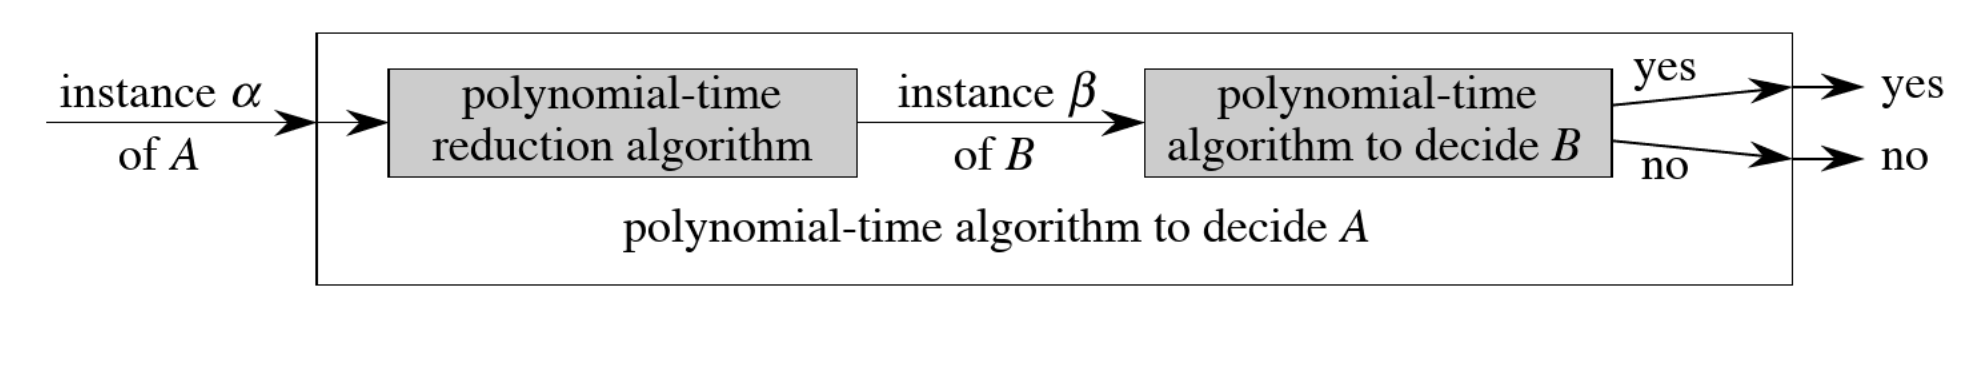
\includegraphics[width=\linewidth]{images/reduction.png}
            \caption{If B can be decided in polynomial-time, then so can A, $A \leq B$}
            \label{fig:reduction}
        \end{figure}
        Additionally, \textbf{Karp reductions} are reductions that use only \textbf{one} call to $B$, whereas \textbf{Turing reductions} allow for \textbf{multiple} calls to $B$. \\ \\ 
        Reductions are also transitive, if $A \leq B$ and $B \leq C$, then $A \leq C$. 
        \begin{defn}
            A problem $A$ is \textbf{NP-hard} if for every problem $B$ in NP, $B \leq A$ (A is at least as hard as all problems in NP). 
        \end{defn}
        \begin{defn}
            A problem $A$ is \textbf{NP-complete} if $A$ is NP-hard and $A$ belongs to NP. 
        \end{defn}
        To show that a problem is NP-complete, we hence just need to show that another NP-complete problem $B$ reduces to $A$, and that $A$ is in NP. 
\section{Approximation Algorithms}
    Algorithm $\mathcal{A}$ is a $\rho$-approximation algorithm for a minimisation problem $\mathcal{P}$ if for every instance $x$ of $\mathcal{P}$ the value $\mathcal{A}(x)$ of the solution produced by $\mathcal{A}$ and the value $OPT(x)$ of the optimal solution satisfy $\mathcal{A}(x) \leq \rho \cdot  OPT(x)$. Approximation algorithms are often used to find a "good enough" solution to an NP-complete problem in polynomial time. \\ \\
    There are three main techniques for constructing approximation algorithms:
    \begin{itemize}
        \item Combinatorial Algorithms
        \item LP Rounding methods
        \begin{itemize}
            \item Express the problem as an Integer Linear Prograam
            \item Relax the integrality constraint to get a regular LP
            \item Since OPT(ILP) $\geq$ OPT(LP) (for minimisation problems), we round LP to an integral solution of the ILP
            \item Argue that the integral solution is not far from OPT(LP)
        \end{itemize}
        \item Randomised Algorithms
    \end{itemize}
    \subsection{2-Approximation Algorithm for MinVertexCover}
    Let $(V, E)$ be an instance of MinVertexCover, i.e. given a graph $G$, what is the minimum set of vertices that cover every edge in $G$? We can form a 2-approximation algorithm:\\ \\
    APPROX-VERTEX-COVER(G)
    \begin{algorithmic}
        \State{$C := \emptyset$}
        \While{$\exists e = (u,v)$ not covered by $C$}
            \State{$C := C \cup \{u,v\}$}
        \EndWhile
        \State{Output $C$}
    \end{algorithmic}
    
    $C$ is a minimum vertex cover as the algorithm only terminates once all vertices have been covered. Furthermore, let $A$ denote the edges that have been picked. Any vertex cover (in particular optimal $C^*$) must include at least one endpoint of each edge in $A$. No two edges in $A$ share an endpoint, as once an edge $e = (u,v)$ has been added to $A$, all other edges that are incident on either $u$ or $v$  will not be considered in the while loop condition (these edges are covered). Hence no two edges in $A$ are covered by the same vertex in $C^*$, meaning that 
    \[ |C^*| \geq |A| \]
    Moreover, as $|C| = 2|A|$ (no edges are incident on one another, so we map pairs of vertices in $C$ to edges in $A$), we have that
    \[ |C| \leq 2|C^*| \]
    \subsection{Linear Program Algorithm for MinVertexCover}
    We introduce variables $\{x_v\}_{v \in V}$ such that $x_v = 1$ if $v$ belongs the the vertex cover, $O$ otherwise. We can then form an ILP:
    \begin{alignat*}{3}
        \text{minimise}  &\quad \sum_{v \in V} x_v && \\
        \text{subject to} 
        &\quad x_u + x_v &&\geq 1 && \quad \text{ for all $(u,v) \in E$} \\
        &\quad x_v &&\in \{0,1\} && \quad \text{ for all $v \in V$}
    \end{alignat*}
    We can also form the relaxed LP:
    \begin{alignat*}{3}
        \text{minimise}  &\quad \sum_{v \in V} x_v && \\
        \text{subject to} 
        &\quad x_u + x_v &&\geq 1 && \quad \text{ for all $(u,v) \in E$} \\
        &\quad x_v &&\geq 0 && \quad \text{ for all $v \in V$} \\ 
        &\quad x_v &&\leq 1 && \quad \text{ for all $v \in V$}
    \end{alignat*}
    We can then round each $v \in V$. If $x_v^* \geq \frac{1}{2}$ then $y_v = 1$ else $y_v = 0$. Then the vertex cover is $C \{ v \ | \ y_v = 1 \}$. We know that this is a VC as by the constraints, at least one of $x_u^*, x_v^* \geq \frac{1}{2}$\\ \\
    We also know that $|C*| \geq \sum_{v \in V}x_v^*$, as the ILP is more constrained that the relaxed LP. Furthermore $y_v \leq 2x_v^*$, so 
    \begin{align*}
        |C| &= \sum_{v \in V} y_v \\
            &\leq 2 \sum_{v \in V} x_v^* \\
            &\leq 2 |C^*|
    \end{align*}
    \subsection{Greedy Algorithm for SetCover}
    Given a set $U$ = $\{ u_1, \ldots, u_n \}$ and a collection of subsets of $U$, $\mathcal{F} = \{ S_1, \ldots, S_m \}$ how can we find the minimum number of sets from $\mathcal{F}$ whose union is $U$? \\ \\
    GREEDY-SET-COVER(G)
    \begin{algorithmic}
        \State{$C := \emptyset$}
        \While{ $\exists$ an element of $U$ not covered by $C$}
            \State{Pick $S \in \mathcal{F}$} that contains the maximum number of uncovered elements
            \State{$C := C \cup \{S\}$}
        \EndWhile
    \end{algorithmic}
    We can see that $C$ is a set cover of $U$. We also claim that $|C| \leq (ln \ n + 1)|C^*|$. At step $t$ of the while loop, let $n_t$ be the number of uncovered elements. There exists a set in $C^*$ that covers at least $\frac{n_t}{|C^*|}$, as otherwise $\bigcup_{S \in C^*} S$ would have less than $n_t$ elements. Hence the set $S$ chosen at this stage of the while loop also covers $\frac{n_t}{|C^*|}$ elements. Hence
    \begin{align*}
        n_{t+1} &\leq n_t - \frac{n_t}{|C^*|} \\ 
                &= (1 - \frac{1}{|C^*|})n_t
    \end{align*} 
    Hence 
    \[ n_t \leq (1 - \frac{1}{|C^*|})^t n \]
    So for $t > |C^*| ln \ n$
    \begin{align*}
        n_t &< (1 - \frac{1}{|C^*|})^{|C^*| ln \ n} n \\ 
            &\leq 1 \tag{Using $1 - \frac{1}{|C^*|} \leq e^{\frac{-1}{|C^*|}}$}
    \end{align*}
    Meaning that after $|C^*| \ ln \ n$ steps, we have fewer than $1$, i.e. $0$ uncovered elements. Hence 
    \begin{align*}
        |C| &\leq |C^*| ln \ n + 1 \\
            &\leq (ln \ n + 1) |C^*|
    \end{align*} 
    \subsection{LP Rounding for SetCover}
    We introduce variables $\{ x_S \}_{S \in \mathcal{F}}$ such that $x_S$ = 1 if $S$ belongs to set cover $C$, otherwise $0$. \\ \\ 
    We can form the ILP:
    \begin{alignat*}{3}
        \text{minimise}  &\quad \sum_{S \in F} x_S && \\
        \text{subject to} 
        &\quad \sum_{S \ : \ u \in S} &&\geq 1 && \quad \text{ for all $u \in U$} \\
        &\quad x_S &&\in \{0,1\} && \quad \text{ for all $S \in F$}
    \end{alignat*}
    And also the relaxed LP:
    \begin{alignat*}{3}
        \text{minimise}  &\quad \sum_{S \in F} x_S && \\
        \text{subject to} 
        &\quad \sum_{S \ : \ u \in S} &&\geq 1 && \quad \text{ for all $u \in U$} \\
        &\quad x_S &&\leq 1 && \quad \text{ for all $S \in F$} \\ 
        &\quad x_S &&\geq 0 && \quad \text{ for all $S \in F$} \\ 
    \end{alignat*}
    We can then round by setting $y_s = 1$ iff $x_S^* \geq \frac{1}{f}$, where $f = max_{u \in U} |\{ S \in \mathcal{F} \ | \ u \in S \}| $ is the maximum frequency of an element in $U$. We can also see that $|C| \leq f \cdot |C^*|$, as for every $S \in \mathcal{F}$ we have that $y_s \leq f x_S^*$, so 
    \begin{align*}
        |C| &= \sum_{S \in F} y_S \\ 
            &\leq f \sum_{S \in \mathcal{F}} x_S^* \\ 
            \leq f \cdot |C^*|
    \end{align*}
    \subsection{$\frac{1}{2}$-Approximation for MaxSAT}
    Given a CNF formula $\phi$, what are the maximum number of clauses that can be satisfied by a variable assignment? \\ \\
    We use a randomisation algorithm for this. Let $V$ be the variables of $\phi$, we set $\sigma(x)$ to be TRUE or FALSE with probability $\frac{1}{2}$. Let $X$ equal the number of satisfied clauses under $\sigma$. \\ \\
    For any clause $c$, denote the number of literals in $c$ by $|c|$. We also say that $X_c$ = 1 if $c$ is satisfied by $\sigma$, and 0 otherwise. We can then see that 
    \[ X = \sum_{c \in C} X_c \]
    By the linearity of expectation, we can see that $\mathbb{E}(X) = \sum_{c \in C} \mathbb{E}[X_c]$. Since we also know that the probability that $c$ is unsatisfied is $1- \frac{1}{2^{|c|}}$,
    \begin{align*}
        \mathbb{E}(X) &= \sum_{c \in C} \mathbb{E}(X_c) \\
                      &= \sum_{c \in C} \mathbb{P}(\text{$c$ is unsatisfied}) \\
                      &= \sum_{c \in C} 1 - \frac{1}{2^{|c|}} \\ 
                      &= \sum_{c \in C} \frac{1}{2} + (\frac{1}{2} - \frac{1}{2^{|c|}}) \\ 
                      &\geq \frac{1}{2}|C|
    \end{align*}
    So we have are guaranteed at least $\frac{|C|}{2}$ clauses to be satisfied in expectation (which means that such an assignment actually exists). We can see by Markov's inequality that the probability of failure (that we do not find such an assignment) is bounded by $\frac{|C|}{|C|+1}$. Let $Y = |C| - X$ be the number of unsatisfied clauses, then
    \begin{align*}
        \mathbb{P}(Y > \frac{|C|}{2}) &= \mathbb{P}(Y \geq \frac{|C|+1}{2}) \\
        &\leq \frac{2}{|C|+1}\mathbb{E}(Y) \\
        &\leq \frac{|C|}{|C+1}
    \end{align*}
    Hence after we have tried the algorithm $10(|C|+1)$ times, we have that
    \begin{align*}
        \mathbb{P}(\text{no success}) &= (\frac{|C|}{|C|+1})^{10(|C|+1)} \\ 
        &= (1 - \frac{1}{|C|+1})^{10(|C|+1)} \\ 
        &\leq e^{-10} \\
        &< 10^{-4}
    \end{align*}

    \subsection{Derandomisation}
        
    
    \section{Fixed Parameter Algorithms}

\end{document}
